%!TEX program = xelatex
%Template created by: Maciej Byczko
\documentclass[a4paper,12pt]{extarticle}  %typ dokumentu

\usepackage{geometry} %poprawienie marginesów
\usepackage{polski} %polskie znaki
\usepackage{graphicx} %grafiki
\usepackage{multirow} % tabele
\usepackage{bigstrut} % tabele
\usepackage{float} %poprawienie pozycji
\usepackage{fancyhdr} % header i footer
\usepackage{hyperref} %tworzenie odnośników, \url{<url>}, \href{<file path, link>}{<text with link>} \pageref{}
\usepackage{slashbox}
\usepackage{longtable}
% \usepackage{multirow}
% \usepackage{tocbibind}
\graphicspath{{pictures/}}
\geometry{margin=0.7in}
\pagestyle{fancy}
\cfoot{Strona \thepage}
\rhead{Strona \thepage}
\lhead{\typdoc}
\setlength{\headheight}{15pt}

%Ustawienie paczki hyperref
\hypersetup{
     colorlinks,
     citecolor=black,
     filecolor=black,
     linkcolor=black,
     urlcolor=black
}


\title{\tytul \\ \small{\opis}}
\author{\tworcy}
\date{\data}

%-----------------------SEKCJA DANYCH----------------------------------
\def\tytul{Technologie Sieciowe - Projekt} %<<< tytuł ćwiczenia
\def\nrcw{} %<<< numer ćwiczenia
\def\data{\today \\ \small{\zajinfo}} %<< data wykonania
\def\prowadzacy{Prowadzący: dr. inż Arkadiusz Grzybowski} %<<<prowadzący
\def\nrgrupy{} %<<<numer grupy
\def\tworcy{Autorzy:\\Karol Baraniecki (252726)\\Maciej Byczko(252747)} %<<< autorzy
\def\zajinfo{PN 14:00 TP\\ Politechnika Wrocławska\\Wydział Informatyki i Telekomunikacji} %<<< informacje dotyczące zajęć
\def\typdoc{} %<<< typ dokumentu tj Sprawozdanie, zadania itp. {Matematyka dyskretna/Sprawozdanie z Miernictwa}
\def\opis{\prowadzacy} %<<< opis który będzie umieszczony pod tytułem w Maketitle
%----------------------------------------------------------------------

\newcommand{\tabc}[1]{
	\textbf{
	\begin{tabular}{c}
		#1
	\end{tabular}
	}
}

\begin{document}
\maketitle
\tableofcontents
\listoftables
\cleardoublepage
\section{Wstęp}
Celem projektu jest zaprojektowanie lokalnej sieci komputerowej dla firmy programistycznej znajdującej się we Wrocławiu.
Sieć musi zostać zaprojektowana zgodnie ze sprecyzowanymi wymaganiami firmy oraz uwzględniać jej przyszły rozwój.
\subsection{Kadra firmy}

Personel firmy składa się z następujących użytkowników:
\begin{itemize}\label{itemize:kadra}
	\item Programiści
	\item Testerzy
	\item Projektanci
	\item Marketing
	\item Księgowość
\end{itemize}
\subsection{Opis siedziby firmy}
Przedsiębiorstwo znajduje się przy ulicy Nowowiejskiej 69\label{address}, składa się z dwóch budynków: dwupiętrowego oraz trzypiętrowego.
% W budynkach znajduje się także odpowiednie wyposażenie (serwery,  drukarki,
% komputery,  kamery  IP,  itp.).
% Firma posiada jeden główny punkt dystrybucyjny (MDF) oraz punkty pośrednie (IDF) w każdym z budynków.
\subsubsection{Lokalizacja firmy na mapie}
\begin{minipage}[c]{0.49\linewidth}

	\begin{figure}[H]
		\centering
		\resizebox*{\textwidth}{!}{
			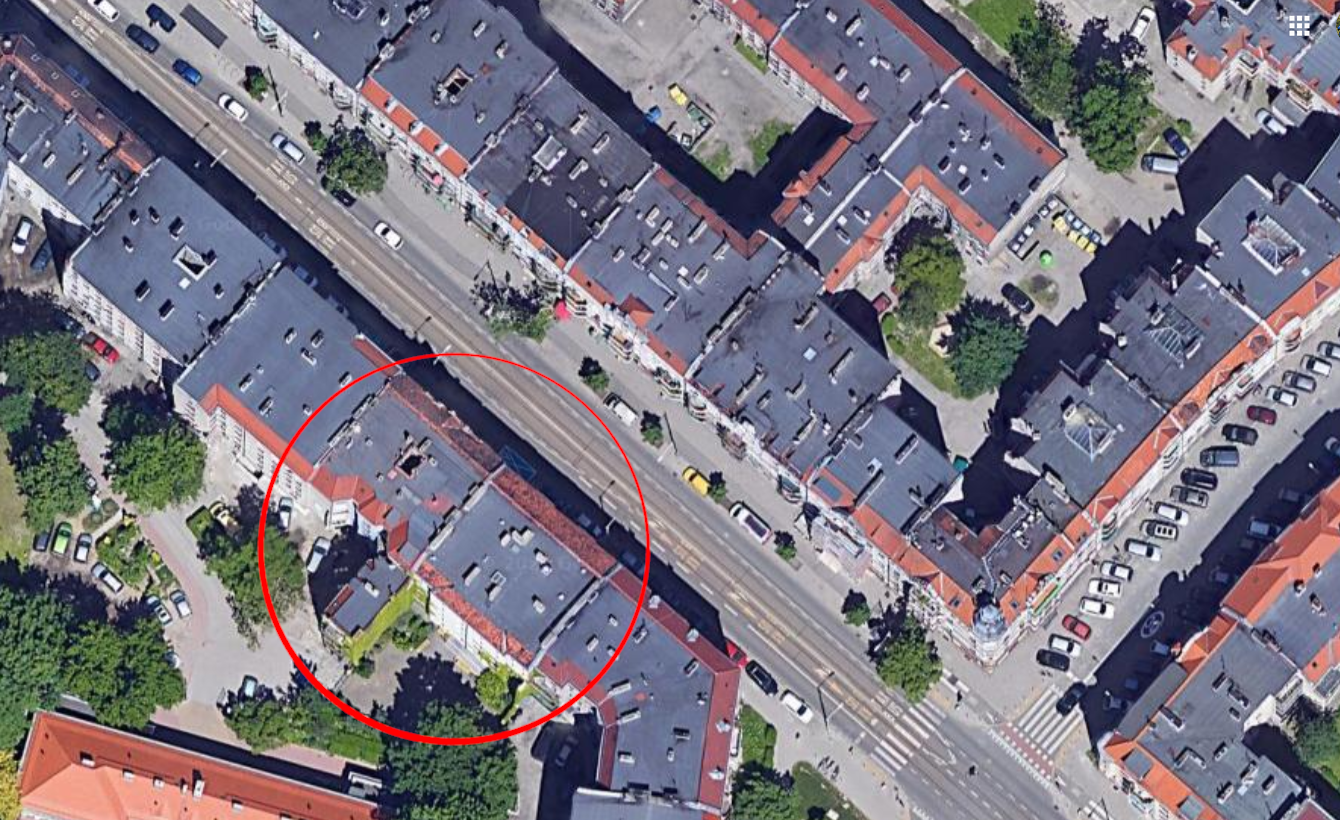
\includegraphics{../pictures/building/building_close.png}
		}
	\end{figure}
\end{minipage}
\begin{minipage}[c]{0.49\linewidth}

	\begin{figure}[H]
		\centering
		\resizebox*{\textwidth}{!}{
			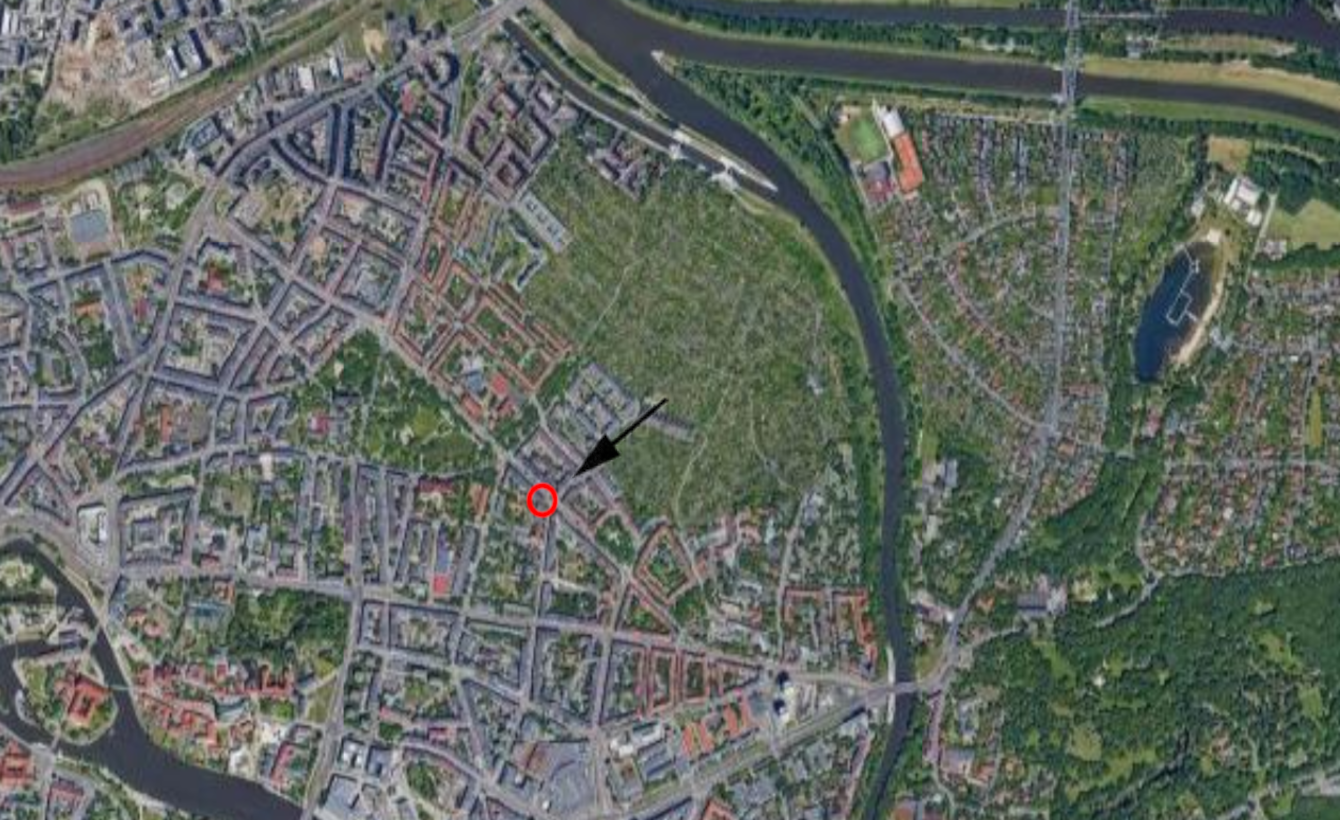
\includegraphics{../pictures/building/building_not_close.png}
		}
	\end{figure}
\end{minipage}
\subsection{Wymagania}
Firma wymaga od nas aby:
\begin{itemize}
	\item Użyta technologia była z rodziny Ethernet,
	\item na wskazanym piętrze każdego budynku ma być dostępna sieć bezprzewodowa (niezbędna instalacja
	      kablowa jest przygotowana),
	\item należy zapewnić dodatkowe porty na przełącznikach (w liczbie 20\% zajętych portów), w związku z
	      przewidywanym wzrostem liczby pracowników (w pomieszczeniach są już zainstalowane
	      dodatkowe gniazda sieciowe),
	\item ruch w ramach grup roboczych ma być separowany z wykorzystaniem sieci VLAN,
	\item należy  zapewnić  dwa  podłączenia  do  Internetu:  podstawowe  oraz  zapasowe,  o  przepustowości
	      adekwatnej do potrzeb przedsiębiorstwa,
	\item podstawowe  łącze  internetowe  ma  zapewniać  gwarancję  minimalnej  przepustowości  równej  co
	      najmniej 40\% średniego przewidywanego przepływu na tym łączu,
	\item kosztorys ma uwzględniać koszt wszystkich urządzeń, podłączenia do Internetu i koszt korzystania z
	      łączy Internetowych w okresie 2 lat
\end{itemize}


%!=========ETAP 2=============


\section{Inwentaryzacja zasobów}
Ilości posiadanych pracowników, oraz urządzeń.
\subsection{Pracownicy}
Pracowników można podzielić na 5 grup roboczych (Patrz \underline{\nameref{itemize:kadra}}).
Każdy z pracowników posiada dostęp do stanowiska pracy na którym znajduje się urządzenie wymagające podłączenia do sieci (w naszym przypadku każdy użytkownik posiada komputer)

\subsubsection{Tabele podziału pracowników}
\begin{table}[H]
	\centering
	\caption{Podział użytkowników na grupy robocze, budynki oraz piętra}
	\vspace{2mm}
	\resizebox{\textwidth}{!}{
		\begin{tabular}{|c|c|c|c|c|c|}
			\cline{2-6}    \multicolumn{1}{c|}{} & \multicolumn{5}{c|}{\textbf{Liczba użytkowników (komputerów)}} \bigstrut                                                                                                                           \\
			\cline{2-6}    \multicolumn{1}{c|}{} & \multicolumn{2}{c|}{\textbf{Budynek 1}}                                  & \multicolumn{3}{c|}{\textbf{Budynek 2}} \bigstrut                                                                       \\\hline
			\textbf{Grupa robocza}               & \textbf{Piętro 1}                                                        & \textbf{Piętro 2}                                 & \textbf{Piętro 1} & \textbf{Piętro 2} & \textbf{Piętro 3} \bigstrut \\\hline
			\textbf{Programiści}                 & 22                                                                       & 6                                                 & 2                 & 19                & 36 \bigstrut                \\\hline
			\textbf{Testerzy}                    & 21                                                                       & 31                                                & 6                 & 13                & 33 \bigstrut                \\\hline
			\textbf{Projektanci}                 & 6                                                                        & 31                                                & 18                & 1                 & 14 \bigstrut                \\\hline
			\textbf{Marketing}                   & 16                                                                       & 28                                                & 7                 & 3                 & 17 \bigstrut                \\\hline
			\textbf{Księgowość}                  & 32                                                                       & 14                                                & 32                & 21                & 15 \bigstrut                \\\hline
		\end{tabular}%
	}
	\label{tab:groups}%
\end{table}%

\begin{table}[H]
	\centering
	\caption{Suma poszczególnych pracowników w firmie wraz z podziałem na grupy robocze}
	\vspace{2mm}
	\begin{tabular}{|c|r|}\hline
		\textbf{Grupa robocza}               & \multicolumn{1}{l|}{\textbf{Suma}} \bigstrut \\\hline
		\textbf{Programiści}                 & 85 \bigstrut                                 \\\hline
		\textbf{Testerzy}                    & 104 \bigstrut                                \\\hline
		\textbf{Projektanci}                 & 70 \bigstrut                                 \\\hline
		\textbf{Marketing}                   & 71 \bigstrut                                 \\\hline
		\textbf{Księgowość}                  & 114 \bigstrut                                \\\hline
		\textbf{Liczba drukarek}             & 12 \bigstrut                                 \\\hline
		\textbf{Suma wszystkich pracowników} & 444 \bigstrut                                \\\hline
	\end{tabular}%
	\label{tab:groups_sum}%
\end{table}%

\subsection{Sprzęt}
Firma jest wyposażona w trzy rodzaje sprzętu:
\begin{itemize}
	\item drukarki
	\item punkty dostępowe WiFi
	\item urządzenia bezprzewodowe
\end{itemize}
Sprzęty te będą używane w sieci lokalnej firmy.
\subsubsection{Tabele podziału urządzeń wspólnych}
\begin{table}[H]
	\centering
	\caption{Podział urządzeń na budynki oraz piętra}
	\vspace{2mm}
	\resizebox{\textwidth}{!}{
		\begin{tabular}{|c|c|c|c|c|c|}
			\cline{2-6}    \multicolumn{1}{c|}{}     & \multicolumn{5}{c|}{\textbf{Liczba urządzeń}} \bigstrut                                                                                                                           \\
			\cline{2-6}    \multicolumn{1}{c|}{}     & \multicolumn{2}{c|}{\textbf{Budynek 1}}                 & \multicolumn{3}{c|}{\textbf{Budynek 2}} \bigstrut                                                                       \\\hline
			\textbf{Urządzenia}                      & \textbf{Piętro 1}                                       & \textbf{Piętro 2}                                 & \textbf{Piętro 1} & \textbf{Piętro 2} & \textbf{Piętro 3} \bigstrut \\\hline
			\textbf{Liczba drukarek}                 & 1                                                       & 2                                                 & 3                 & 3                 & 3 \bigstrut                 \\\hline
			\textbf{Liczba punktów dostępowych WiFi} & 0                                                       & 0                                                 & 1                 & 0                 & 3 \bigstrut                 \\\hline
			\textbf{Liczba urządzeń bezprzewodowych} & 0                                                       & 0                                                 & 6                 & 0                 & 17 \bigstrut                \\\hline
		\end{tabular}%
	}
	\label{tab:devices}%
\end{table}%

\begin{table}[H]
	\centering
	\caption{Suma poszczególnych urządzeń w firmie}
	\vspace{2mm}
	\begin{tabular}{|c|r|}\hline
		\textbf{Urządzenia}                      & \multicolumn{1}{l|}{\textbf{Suma}} \bigstrut \\\hline
		\textbf{Liczba drukarek}                 & 12 \bigstrut                                 \\\hline
		\textbf{Liczba punktów dostępowych WiFi} & 4 \bigstrut                                  \\\hline
		\textbf{Liczba urządzeń bezprzewodowych} & 23 \bigstrut                                 \\\hline
		\textbf{Suma wszystkich urządzeń}        & 39 \bigstrut                                 \\\hline
	\end{tabular}%
	\label{tab:devices_sum}%
\end{table}%

% \subsection{Wymagania przepływowe pomiędzy pracownikami a serwerami lokalnymi}


\subsection{Serwery}
Firma posiada dwa serwery lokalne. Serwer lokalny 1 jest używany przez:
\begin{itemize}
	\item Testerów,
	\item Marketing,
	\item WiFi
\end{itemize}
Serwer lokalny 2 jest używany przez każdą grupę roboczą z wyłączeniem zespołu Marketingu.
\begin{table}[H]
	\centering
	\caption{Prognozowany ruch do internetu}
	\vspace{2mm}
	\resizebox{\textwidth}{!}{
		\begin{tabular}{|c|c|c|c|}
			\cline{2-4}    \multicolumn{1}{c|}{} & \multicolumn{3}{c|}{\textbf{Transfer do\textbackslash{}z Internetu na jedną sesję (internautę) [kb/s] }} \bigstrut                                                                        \\\hline
			\textbf{Serwery internetowe}         & \textbf{Do Internetu}                                                                                              & \textbf{Z Internetu} & \textbf{Liczba jednoczesnych sesji} \bigstrut \\\hline
			\textbf{Serwer WWW}                  & 50                                                                                                                 & 15                   & 49 \bigstrut                                  \\\hline
			\textbf{Serwer FTP}                  & 210                                                                                                                & 90                   & 4 \bigstrut                                   \\\hline
		\end{tabular}%
	}
	\label{tab:www_traffic}%
\end{table}%
\subsection{Aplikacje}
Dla każdej grupy użytkowników został zdefiniowany również przepływ do i z internetu z podziałem na poszczególne typy aplikacji, firma zapewnia również dostęp do sieci WiFi.
\begin{table}[H]
	\centering
	\caption{Wymagania dotyczące przepływu przez aplikacje}
	\vspace{2mm}
	\resizebox{\textwidth}{!}{
		\begin{tabular}{|c|c|c|c|c|c|}\hline
			\multicolumn{6}{|c|}{\textbf{Transfer z/do Internetu (down \textbackslash{} up) [kb/s]}} \bigstrut                                                                               \\\hline
			\textbf{\backslashbox{Grupa rob.}{Aplikacja}} & \textbf{Przeglądarka} & \textbf{Wideokonferencja} & \textbf{VoIP}        & \textbf{Klient\_FTP} & \textbf{Komunikator} \bigstrut \\\hline
			\textbf{Programiści}                          & 0\textbackslash{}0    & 0\textbackslash{}0        & 20\textbackslash{}20 & 77\textbackslash{}18 & 15\textbackslash{}15 \bigstrut \\\hline
			\textbf{Testerzy}                             & 0\textbackslash{}0    & 40\textbackslash{}40      & 0\textbackslash{}0   & 0\textbackslash{}0   & 15\textbackslash{}15 \bigstrut \\\hline
			\textbf{Projektanci}                          & 65\textbackslash{}10  & 0\textbackslash{}0        & 20\textbackslash{}20 & 45\textbackslash{}11 & 15\textbackslash{}15 \bigstrut \\\hline
			\textbf{Marketing}                            & 60\textbackslash{}10  & 40\textbackslash{}40      & 20\textbackslash{}20 & 0\textbackslash{}0   & 15\textbackslash{}15 \bigstrut \\\hline
			\textbf{Księgowość}                           & 35\textbackslash{}10  & 40\textbackslash{}40      & 20\textbackslash{}20 & 0\textbackslash{}0   & 0\textbackslash{}0 \bigstrut   \\\hline
			\textbf{WiFi}                                 & 78\textbackslash{}10  & 40\textbackslash{}40      & 20\textbackslash{}20 & 49\textbackslash{}14 & 15\textbackslash{}15 \bigstrut \\\hline
		\end{tabular}%
	}
	\label{tab:apps}%
\end{table}%

\section{Analiza potrzeb użytkowników}
Wymagania potrzebne dla pracowników w celu sprawnej pracy w firmie.
\subsection{Pracownicy oraz wykorzystywane oprogramowanie}
W zależności od typu stanowiska wymagana jest różna jakość usług sieciowych. Jest to związane z tym że wykorzystywane jest różne oprogramowanie. Każda aplikacja działa w sposób indywidualny, niektóre wymagają bardzo stabilnego łącza, bądź bezpieczeństwa połączenia.
Na podstawie \underline{\hyperref[tab:usage]{tabeli 7}} można wywnioskować wymagania oraz zużycie każdej grupy roboczej, rozpatrzymy każde stanowisko z osobna:
\begin{itemize}
	\item Programiści - wymagają przede wszystkim szybkiego połączenia ze względu na znaczne użycie usługi FTP.
	\item Testerzy - wymagają szybkiego i niezawodnego łącza ze względu na wideokonferencje.
	\item Projektanci - wymagają bezpiecznego oraz szybkiego połączenia ze względu na usługę FTP oraz używanie przeglądarki.
	\item Marketing - wymagają stabilnego łącza ze względu na wideokonferencję, bezpieczeństwo także się przyda ze względu na użycie przeglądarki.
	\item Księgowość - głównie wymagają stabilnego łącza ze względu na wideokonferencje, używają także przeglądarki więc łącze musi być bezpieczne.
	      % \item WiFi - oferuje multum usług więc powinno mieć głównie bezpieczeństwo połączenia,  
\end{itemize}

\subsection{Łącza szkieletowe}
% \subsection{Łącza do serwerów i drukarek}
\begin{table}[H]
	\centering
	\caption{Wymagania dotyczące przepływów lokalnych (na jednego użytkownika)}
	\vspace{2mm}
	\resizebox{\textwidth}{!}{
		\begin{tabular}{|c|c|c|c|}
			\cline{2-4}    \multicolumn{1}{c|}{}       & \multicolumn{3}{c|}{\textbf{Transfer do serwerów lokalnych i drukarek (down \textbackslash{} up) [kb/s]}} \bigstrut                                                            \\\hline
			\textbf{\backslashbox{Grupa rob.}{Serwer}} & \textbf{Serwer1}                                                                                                    & \textbf{Serwer2}       & \textbf{Drukarka} \bigstrut     \\\hline
			\textbf{Programiści}                       & 0\textbackslash{}0                                                                                                  & 750\textbackslash{}700 & 10\textbackslash{}120 \bigstrut \\\hline
			\textbf{Testerzy}                          & 700\textbackslash{}350                                                                                              & 450\textbackslash{}100 & 10\textbackslash{}130 \bigstrut \\\hline
			\textbf{Projektanci}                       & 0\textbackslash{}0                                                                                                  & 350\textbackslash{}200 & 10\textbackslash{}190 \bigstrut \\\hline
			\textbf{Marketing}                         & 150\textbackslash{}200                                                                                              & 0\textbackslash{}0     & 10\textbackslash{}140 \bigstrut \\\hline
			\textbf{Księgowość}                        & 0\textbackslash{}0                                                                                                  & 450\textbackslash{}250 & 10\textbackslash{}130 \bigstrut \\\hline
			\textbf{WiFi}                              & 50\textbackslash{}250                                                                                               & 100\textbackslash{}250 & 10\textbackslash{}120 \bigstrut \\\hline
		\end{tabular}%
	}
	\label{tab:usage}%
\end{table}%
Aby uzyskać szacowane łącza według grup roboczych na jednego użytkownika należy zsumować cały ruch generowany przez jednego użytkownika danej grupy.
Wyliczenia zostały wykonane na podstawie poprzednich tabel.

\begin{table}[H]
	\centering
	\caption{Szacowane wykorzystywanie łącza przez pojedynczego użytkownika z danych grup roboczych}
	\vspace{2mm}
	\resizebox{\textwidth}{!}{
		\begin{tabular}{|c|c|c|c|c|c|c|}
			\hline
			\multirow{3}[4]{*}{\textbf{Użytkownik}} & \multicolumn{2}{c|}{\textbf{Lokalnie}} & \multicolumn{2}{c|}{\textbf{Internet}} & \multicolumn{2}{c|}{\textbf{Suma}} \bigstrut                                                                    \\
			\cline{2-7}                             & \textbf{down}                          & \textbf{up}                            & \textbf{down}                                & \textbf{up}     & \textbf{down}   & \textbf{up} \bigstrut[t]     \\
			                                        & \textbf{[kb/s]}                        & \textbf{[kb/s]}                        & \textbf{[kb/s]}                              & \textbf{[kb/s]} & \textbf{[kb/s]} & \textbf{[kb/s]} \bigstrut[b] \\\hline
			\textbf{Programiści}                    & 760                                    & 820                                    & 112                                          & 53              & 872             & 873 \bigstrut                \\\hline
			\textbf{Testerzy}                       & 1160                                   & 580                                    & 55                                           & 55              & 1215            & 635 \bigstrut                \\\hline
			\textbf{Projektanci}                    & 360                                    & 390                                    & 145                                          & 56              & 505             & 446 \bigstrut                \\\hline
			\textbf{Marketing}                      & 160                                    & 340                                    & 135                                          & 85              & 295             & 425 \bigstrut                \\\hline
			\textbf{Księgowość}                     & 460                                    & 380                                    & 95                                           & 70              & 555             & 450 \bigstrut                \\\hline
			\textbf{WiFi}                           & 160                                    & 620                                    & 202                                          & 99              & 362             & 719 \bigstrut                \\\hline
		\end{tabular}%
	}
	\label{tab:user_usage}%
\end{table}%
\textbf{Przykład obliczeń:}\\
Wyliczenia na podstawie grupy roboczej \emph{Programiści} z \underline{\hyperref[tab:apps]{tabeli 7}}:
\begin{itemize}
	\item Pobieranie z Internetu: $0+0+20+77+15=112[kb/s]$
	\item Wysyłanie do Internetu: $0+0+20+18+15=53[kb/s]$
	\item Pobieranie lokalne: $0+750+10=760[kb/s]$
	\item Wysyłanie lokalne:$0+700+120=820[kb/s]$
	\item Suma pobierania: $112+760=872[kb/s]$
	\item Suma wysyłania: $53+820=873[kb/s]$
\end{itemize}
Grupy o największym korzystaniu z sieci to:
\begin{itemize}
	\item Testerzy (Pobieranie) - $1215[kb/s] \approx 1.19[Mb/s]$
	\item Programiści (Wysyłanie) - $873[kb/s] \approx 0.85[Mb/s]$ %(po zaokrągleniu w górę $0.86[Mb/s]$ aby nie było straty na łączu)
\end{itemize}
Aby uzyskać szacowany ruch generowany przez pracowników danego piętra,
należy pomnożyć ruch przypadający na jednego pracownika z
\underline{\hyperref[tab:user_usage]{tabeli 8}} przez liczbę pracowników danej grupy roboczej na określonym piętrze (\underline{\hyperref[tab:groups]{tabela 1}})
% \subsubsection{Szacowany pobór danych}
% Table generated by Excel2LaTeX from sheet ,Sheet1,
% Table generated by Excel2LaTeX from sheet ,Sheet1,
\begin{table}[H]
	\centering
	\caption{Szacowany pobór danych}
	\vspace{2mm}
	\resizebox{\textwidth}{!}{
		\begin{tabular}{|c|c|c|c|c|c|}
			\hline
			\multirow{2}[4]{*}{\textbf{Użytkownik}} & \multicolumn{2}{c|}{\textbf{Budynek 1}} & \multicolumn{3}{c|}{\textbf{Budynek 2}} \bigstrut                                                                       \\
			\cline{2-6}                             & \textbf{Piętro 1}                       & \textbf{Piętro 2}                                 & \textbf{Piętro 1} & \textbf{Piętro 2} & \textbf{Piętro 3} \bigstrut \\
			\hline
			\textbf{Programiści}                    & 19184                                   & 5232                                              & 1744              & 16568             & 31392 \bigstrut             \\
			\hline
			\textbf{Testerzy}                       & 25515                                   & 37665                                             & 7290              & 15795             & 40095 \bigstrut             \\
			\hline
			\textbf{Projektanci}                    & 3030                                    & 15655                                             & 9090              & 505               & 7070 \bigstrut              \\
			\hline
			\textbf{Marketing}                      & 4720                                    & 8260                                              & 2065              & 885               & 5015 \bigstrut              \\
			\hline
			\textbf{Księgowość}                     & 17760                                   & 7770                                              & 17760             & 11655             & 8325 \bigstrut              \\
			\hline
			\textbf{Suma}                           & 70209                                   & 74582                                             & 37949             & 45408             & 91897 \bigstrut             \\
			\hline
		\end{tabular}%
	}
	\label{tab:user_download}%
\end{table}%

% Table generated by Excel2LaTeX from sheet ,Sheet1,
\begin{table}[H]
	\centering
	\caption{Szacowany przesył danych
		\vspace{2mm}}
	\resizebox{\textwidth}{!}{
		\begin{tabular}{|c|c|c|c|c|c|}
			\hline
			\multirow{2}[4]{*}{\textbf{Użytkownik}} & \multicolumn{2}{c|}{\textbf{Budynek 1}} & \multicolumn{3}{c|}{\textbf{Budynek 2}} \bigstrut                                                                       \\
			\cline{2-6}                             & \textbf{Piętro 1}                       & \textbf{Piętro 2}                                 & \textbf{Piętro 1} & \textbf{Piętro 2} & \textbf{Piętro 3} \bigstrut \\
			\hline
			\textbf{Programiści}                    & 19206                                   & 5238                                              & 1746              & 16587             & 31428 \bigstrut             \\
			\hline
			\textbf{Testerzy}                       & 13335                                   & 19685                                             & 3810              & 8255              & 20955 \bigstrut             \\
			\hline
			\textbf{Projektanci}                    & 2676                                    & 13826                                             & 8028              & 446               & 6244 \bigstrut              \\
			\hline
			\textbf{Marketing}                      & 6800                                    & 11900                                             & 2975              & 1275              & 7225 \bigstrut              \\
			\hline
			\textbf{Księgowość}                     & 14400                                   & 6300                                              & 14400             & 9450              & 6750 \bigstrut              \\
			\hline
			\textbf{Suma}                           & 56417                                   & 56949                                             & 30959             & 36013             & 72602 \bigstrut             \\
			\hline
		\end{tabular}%
	}
	\label{tab:user_upload}%
\end{table}%
\textbf{Przykład obliczeń:}\\
Wyliczenia na podstawie grupy roboczej \emph{Programiści} z \underline{\hyperref[tab:user_usage]{tabeli 8}} oraz \underline{\hyperref[tab:groups]{tabeli 1}}:\\
Dla piętra 1:
\begin{itemize}
	\item Pobieranie: $872*22=19184[kb/s]\approx 18.74[Mb/s]$
	\item Wysyłanie: $873*22=19206[kb/s]\approx 18.76[Mb/s]$
\end{itemize}
Według przeprowadzonych obliczeń najbardziej wymagające jest \textbf{Piętro 3 w budynku 2}.
\begin{itemize}
	\item Pobieranie: $91897[kb/s]\approx89.75[Mb/s]$
	\item Wysyłanie: $72602[kb/s]\approx70.90[Mb/s]$
\end{itemize}
\subsection{Obciążenie poszczególnych punktów dystrybucyjnych}
% Table generated by Excel2LaTeX from sheet ,Sheet1,
\begin{table}[H]
	\centering
	\caption{Punkty dystrybucyjne i ich obciążenie}
	\resizebox{\textwidth}{!}{
		\begin{tabular}{|c|c|c|c|c|}
			\hline
			\multicolumn{3}{|c|}{\textbf{Punkty dystrybucyjne}} & \multicolumn{2}{c|}{\textbf{Transmisja}} \bigstrut                                                                                                                   \\
			\hline
			\textbf{Oznaczenie}                                 & \textbf{Lokalizacja}                               & \textbf{Podłączone punkty abonenckie} & \textbf{Pobór danych [Mb/s]} & \textbf{Przesył danych [Mb/s]} \bigstrut \\
			\hline
			\textbf{MDF}                                        & Bud. 2, Piętro 2                                   & Bud. 2, Piętro 2,1,                   & 312.54                       & 247.01 \bigstrut                         \\
			\hline
			\textbf{IDF1}                                       & Bud. 2, Piętro 3                                   & Bud. 2, Piętro 3,                     & 89.74                        & 70.90 \bigstrut                          \\
			\hline
			\textbf{IDF2}                                       & Bud. 1, Piętro 1                                   & Bud. 1                                & 141.40                       & 110.71 \bigstrut                         \\
			\hline
		\end{tabular}%
	}
	\label{tab:distribution}%
\end{table}%
Na podstawie powyższej tabeli możemy określić że największe obciążenie sieci będzie wynosić kolejno:
Pobór w wysokości 312.54[Mb/s] oraz Przesył w wysokości 247.01[Mb/s],
zatem te wartości uznajemy za wymagania naszej sieci.
\subsection{Łącza do serwerów i drukarek}
Aby uzyskać przepustowości połączeń do serwerów lokalnych oraz drukarek
(zakładając, że są dostępne dla dużej ilości użytkowników jednocześnie)
należy pomnożyć ilość pracowników każdej z grup roboczych (\href{tab:groups_sum}{Tabela 2})
przez wymaganą szybkość połączenia z danym serwerem (\underline{\href{tab:usage}{Tabela 7}}).
Tak uzyskane wyniki przedstawiamy w tabeli reprezentującej przepustowości dla każdej z grup
roboczych oraz ich łączną sumę:
% Table generated by Excel2LaTeX from sheet ,Sheet1,
\begin{table}[H]
	\centering
	\caption{Szacowane przepustowości połączeń poboru danych z serwerów i drukarek}
	\resizebox{\textwidth}{!}{
		\begin{tabular}{|c|c|c|c|c|}
			\hline
			\textbf{\backslashbox{Grupa rob.}{Serwer}} & \textbf{Serwer} 1 & \textbf{Serwer} 2 & \textbf{Drukarka} & \textbf{suma} \bigstrut \\
			\hline
			\textbf{Programiści}                       & 0                 & 63750             & 850               & 64600 \bigstrut         \\
			\hline
			\textbf{Testerzy}                          & 72800             & 46800             & 1040              & 120640 \bigstrut        \\
			\hline
			\textbf{Projektanci}                       & 0                 & 24500             & 700               & 25200 \bigstrut         \\
			\hline
			\textbf{Marketing}                         & 10650             & 0                 & 710               & 11360 \bigstrut         \\
			\hline
			\textbf{Księgowość}                        & 0                 & 51300             & 1140              & 52440 \bigstrut         \\
			\hline
			\textbf{WiFi}                              & 200               & 400               & 40                & 640 \bigstrut           \\
			\hline
		\end{tabular}%
	}
	\label{tab:server_download}%
\end{table}%
\begin{table}[H]
	\centering
	\caption{Szacowane przepustowości przesyłu danych do serwerów i drukarek}
	\resizebox{\textwidth}{!}{
		\begin{tabular}{|c|c|c|c|c|}
			\hline
			\textbf{\backslashbox{Grupa rob.}{Serwer}} & \textbf{Serwer} 1 & \textbf{Serwer} 2 & \textbf{Drukarka} & \textbf{suma} \bigstrut \\
			\hline
			\textbf{Programiści}                       & 0                 & 59500             & 10200             & 69700 \bigstrut         \\
			\hline
			\textbf{Testerzy}                          & 36400             & 10400             & 13520             & 60320 \bigstrut         \\
			\hline
			\textbf{Projektanci}                       & 0                 & 14000             & 13300             & 27300 \bigstrut         \\
			\hline
			\textbf{Marketing}                         & 14200             & 0                 & 9940              & 24140 \bigstrut         \\
			\hline
			\textbf{Księgowość}                        & 0                 & 28500             & 14820             & 43320 \bigstrut         \\
			\hline
			\textbf{WiFi}                              & 1000              & 1000              & 480               & 2480 \bigstrut          \\
			\hline
		\end{tabular}%
	}
	\label{tab:server_upload}%
\end{table}%

\subsection{Łącza do internetu}
Łącze internetowe w firmie będzie wykorzystywane przez aplikacje pracowników oraz z
zewnątrz do dostępu do Serwera WWW oraz Serwera Pocztowego.
Aby obliczyć wykorzystanie łącza internetowego należy pomnożyć przepustowości
wymagane dla danych aplikacji (Tabela \underline{\href{tab:apps}{Tabela 6}}) przez ilość pracowników w każdej
z grup roboczych (\underline{\href{tab:groups_sum}{Tabela 2}} i \underline{\href{tab:devices_sum}{Tabela 4}}):
% Table generated by Excel2LaTeX from sheet ,Sheet1,
\begin{table}[H]
	\centering
	\caption{Pobór danych przez aplikacje $[kb/s]$}
	\resizebox{\textwidth}{!}{
		\begin{tabular}{|c|c|c|c|c|c|c|}
			\cline{1-6}    \textbf{Grupa rob./Serwer} & \textbf{Przeglądarka} & \textbf{Wideokonferencja} & \textbf{VoIP} & \textbf{Klient FTP} & \textbf{Komunikator} & \multicolumn{1}{c}{} \bigstrut  \\
			\cline{1-6}    \textbf{Programiści}       & 0                     & 0                         & 1700          & 6545                & 1275                 & \multicolumn{1}{c}{} \bigstrut  \\
			\cline{1-6}    \textbf{Testerzy}          & 0                     & 4160                      & 0             & 0                   & 1560                 & \multicolumn{1}{c}{} \bigstrut  \\
			\cline{1-6}    \textbf{Projektanci}       & 4550                  & 0                         & 1400          & 3150                & 1050                 & \multicolumn{1}{c}{} \bigstrut  \\
			\cline{1-6}    \textbf{Marketing}         & 4260                  & 2840                      & 1420          & 0                   & 1065                 & \multicolumn{1}{c}{} \bigstrut  \\
			\cline{1-6}    \textbf{Księgowość}        & 3990                  & 4560                      & 2280          & 0                   & 0                    & \multicolumn{1}{c}{} \bigstrut  \\
			\hline
			\textbf{WiFi}                             & 312                   & 160                       & 80            & 196                 & 60                   & \textbf{Suma końcowa} \bigstrut \\
			\hline
			\textbf{Suma}                             & 13112                 & 11720                     & 6880          & 9891                & 5010                 & 46613 \bigstrut                 \\
			\hline
		\end{tabular}%
	}
	\label{tab:app_usage_download}%

\end{table}%

% Table generated by Excel2LaTeX from sheet ,Sheet1,
\begin{table}[H]
	\centering
	\caption{Przesył danych przez aplikacje $[kb/s]$}
	\resizebox{\textwidth}{!}{
		\begin{tabular}{|c|c|c|c|c|c|c|}
			\cline{1-6}    \textbf{Grupa rob./Serwer} & \textbf{Przeglądarka} & \textbf{Wideokonferencja} & \textbf{VoIP} & \textbf{Klient FTP} & \textbf{Komunikator} & \multicolumn{1}{c}{} \bigstrut  \\
			\cline{1-6}    \textbf{Programiści}       & 0                     & 0                         & 1700          & 1530                & 1275                 & \multicolumn{1}{c}{} \bigstrut  \\
			\cline{1-6}    \textbf{Testerzy}          & 0                     & 4160                      & 0             & 0                   & 1560                 & \multicolumn{1}{c}{} \bigstrut  \\
			\cline{1-6}    \textbf{Projektanci}       & 700                   & 0                         & 1400          & 770                 & 1050                 & \multicolumn{1}{c}{} \bigstrut  \\
			\cline{1-6}    \textbf{Marketing}         & 710                   & 2840                      & 1420          & 0                   & 1065                 & \multicolumn{1}{c}{} \bigstrut  \\
			\cline{1-6}    \textbf{Księgowość}        & 1140                  & 4560                      & 2280          & 0                   & 0                    & \multicolumn{1}{c}{} \bigstrut  \\
			\hline
			\textbf{WiFi}                             & 40                    & 160                       & 80            & 56                  & 60                   & \textbf{Suma końcowa} \bigstrut \\
			\hline
			\textbf{Suma}                             & 2590                  & 11720                     & 6880          & 2356                & 5010                 & 28556 \bigstrut                 \\
			\hline
		\end{tabular}%
	}
	\label{tab:app_uasge_upload}%

\end{table}%

% Table generated by Excel2LaTeX from sheet ,Sheet1,
\begin{table}[H]
	\centering
	\caption{Szacowane łącze internetowe serwerów}
	\resizebox{\textwidth}{!}{
		\begin{tabular}{|c|c|c|}
			\hline
			\textbf{\backslashbox{Serwery internetowe}{Transfer} } & \textbf{Download [kb/s]} & \textbf{Upload [kb/s]} \bigstrut \\
			\hline
			\textbf{Serwer WWW}                                    & 735                      & 2450 \bigstrut                   \\
			\hline
			\textbf{Serwer FTP}                                    & 360                      & 840 \bigstrut                    \\
			\hline
			\textbf{Suma}                                          & 1095                     & 3290 \bigstrut                   \\
			\hline
		\end{tabular}%
	}
	\label{tab:usage_server}%
\end{table}%

Podsumowując łącze potrzebne firmie wynosi:
\begin{itemize}
	\item Pobór danych - 46613 + 1095 = 47708 [kb/s] $\approx$ 46.59 [Mb/s]
	\item Wysył danych - 28556 + 3290 = 31846 [kb/s] $\approx$ 31.10 [Mb/s]
\end{itemize}

\section{Założenia projektowe}
Założenia na podstawie których wybierzemy dostawców oraz zaplanujemy wstępne zabezpieczenia.
\subsection{Sieć LAN}
W projekcie wyróżniamy podział na bezprzewodową sieć LAN
(technologia 802.11n) oraz przewodową w technologii
Fast Ethernet oraz Gigabit Ethernet.
Zakładamy, że sieć bezprzewodowa ma obsłużyć jednocześnie
23 urządzenia. Zasięg sieci bezprzewodowej ma obejmować
wszystkie budynki firmy.
Serwery zostaną umieszczone na tym samym piętrze co MDF.

\subsection{Łącze do internetu}

Na podstawie wcześniejszych obliczeń i wzięcia pod uwagę
ewentualnego rozwoju sieci* wymagane łącze musi mieć
następujące parametry:\\

\textbf{Upload 32 Mb/s} i \textbf{Download 47 Mb/s}.\\

Oczywistym jest, że stacje robocze nie wykorzystują przez
cały czas wcześniej oszacowanej przepustowości,
ale ważne jest aby uwzględnić taką możliwość.

Pod naszym \underline{\href{address}{adresem}} mamy kilka dostawców internetu i
w celu zapewnienia niezawodności wykorzystane zostaną
usługi internetowe dwóch z nich:
\textbf{UPC} oraz \textbf{Netia}.
W momencie kiedy nie ma awarii sieci można rozdzielić
ruch internetowy na dwa łącza.  W ten sposób maksymalizujemy
dostępną przepustowość. Jeżeli dojdzie do awarii sieci to
wykorzystujemy pozostałe dostępne łącze. W przypadku awarii jednego z dostawców całe obciążenie łącza
zostanie przekazane na działające połączenie.
\subsection{Zabezpieczenia sieci}
Dla zabezpieczenia sieci nakładamy na nią następujące ograniczenia:
\begin{itemize}
	\item Serwer lokalny 1 jest używany wyłącznie przez Testerów, Dział Marketingu oraz poprzez WiFi.
	\item Serwer lokalny 2 może być użyty przez wszystkich, poza Działem Marketingu.
	\item Testerzy z protokołu SSH, który szyfruje przesyłane dane.
	\item Sieć będzie zawierała firewall ustawiony na routerze łączącym z internetem, który pozwoli na monitorowanie i filtrowanie pakietów sieciowych.
	\item Serwery WWW i FTP będą umieszczone w strefie zdemilitaryzowanej ze względów bezpieczeństwa.
	\item W sieci będzie stosowana filtracja adresów MAC w celu dodatkowego zabezpieczenia przed niepowołanym dostępem.
	\item Sieć WiFi będzie zabezpieczona hasłem oraz protokołem WPA2-PSK, aby szyfrować przesyłane dane.
	\item Kable zostaną położone w podłodze technicznej w celu uniemożliwienia dostępu z zewnątrz.
\end{itemize}

\section{Projekt sieci}
\subsection{Projekt logiczny sieci wraz z opisem koncepcji rozwiązania i uzasadnieniem}
\begin{figure}[H]
	\centering
	\resizebox*{0.9\textwidth}{!}{
		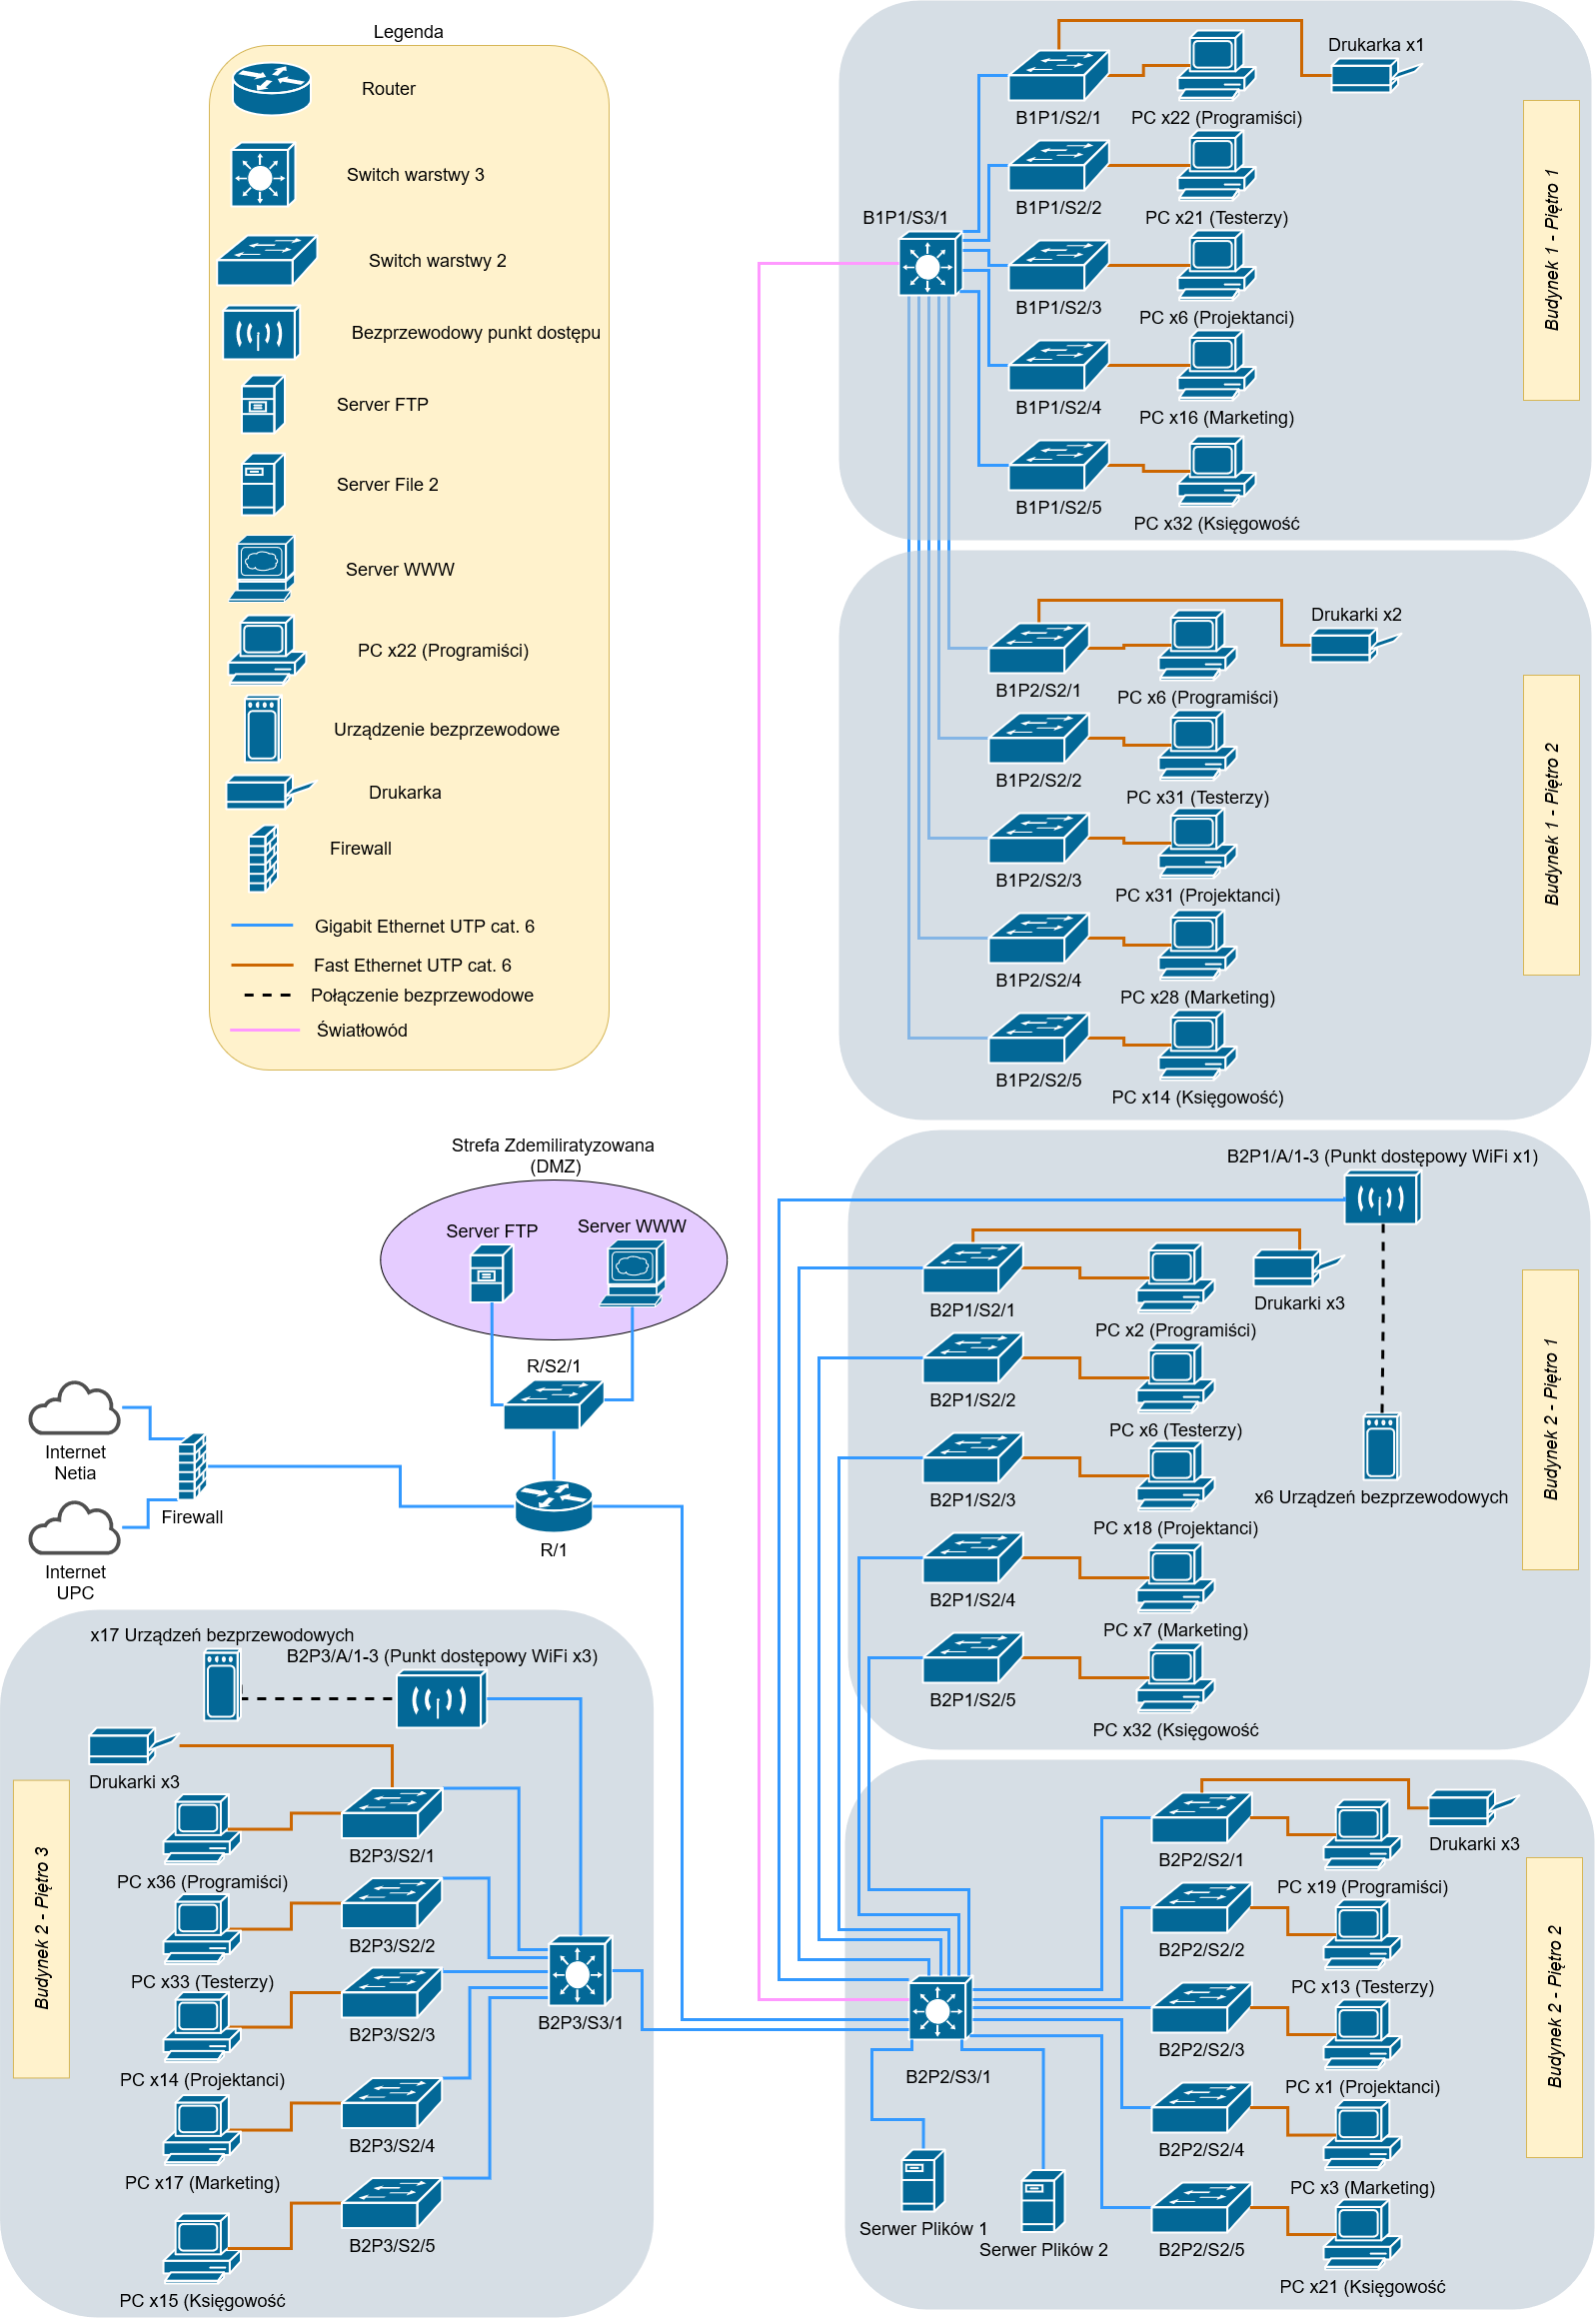
\includegraphics{../pictures/TS_Network_Logic.drawio.png}
	}
\end{figure}
\cleardoublepage
\subsubsection{Podział na sieci VLAN}
Pomijamy VLAN 1 gdyż to jest sieć domyślna, dlatego zaczynamy od VLAN 2
\begin{itemize}
	\item VLAN 2 - Programiści
	\item VLAN 3 - Testerzy
	\item VLAN 4 - Projektanci
	\item VLAN 5 - Marketing
	\item VLAN 6 - Księgowość
	\item VLAN 7 - WiFi
	\item VLAN 8 - Drukarki
	\item VLAN 9 - Serwery FTP oraz WWWW
\end{itemize}
\subsubsection{Opis oznaczeń urządzeń sieciowych}
\textbf{BXPY/T/N}
\begin{itemize}
	% \item DF - Punkt dystrybucyjny
	\item BXPY - Budynek X i piętro Y
	\item T - typ urządzenia
	      \begin{itemize}
		      \item R - Router
		      \item S2 - Switch warstwy drugiej
		      \item S3 - Switch warstwy trzeciej
		      \item A - Access point (punkt dostępu WiFi)
	      \end{itemize}
	\item N - Numer urządzenia sieciowego
\end{itemize}
\subsubsection{Przykładowy odczyt kodu}
\emph{(Kod czytamy od tyłu)}\\
\textbf{B2P2/S2/1} - Switch nr.1 warstwy drugiej znajdujący się na piętrze drugim w budynku drugim.
\subsubsection{Opis oznaczeń urządzeń końcowych}
\textbf{XXX/BXPY/N}
\begin{itemize}
	\item XXX
	      \subitem ITE - komputer Programisty
	      \subitem TES - komputer Testera
	      \subitem PRO - komputer Projektanta
	      \subitem MAR - komputer Działu Marketingu
	      \subitem KSI - komputer Księgowości
	      \subitem DRU - Drukarka
	      \subitem UBE - Urządzenie bezprzewodowe
	\item BXPY - budynek nr X i piętro nr Y
	\item N - numer urządzenia końcowego
\end{itemize}

\subsection{Wybór urządzeń sieciowych}
\subsubsection{Urządzenia aktywne}
\begin{itemize}
	\item Router - Cisco ISR4221/K9
	\item Przełącznik warstwy 3 (MDF) - Cisco Catalyst 2960X-24TS-LL
	\item przełącznik warstwy 3 (IDF-y) - Cisco SF350-48
	\item Przełącznik warstwy 2 - Cisco SF220-48
	\item Punkt dostępu - TP-LINK EAP265 HD
\end{itemize}
W naszym projekcie wybraliśmy \textbf{router Cisco ISR4221/K9} ze względu na dobry stosunek
ceny do jakości. \\

Do obsługi ruchu pomiędzy budynkami oraz połączenia routera do reszty sieci zostaną użyte
\textbf{przełącznik Cisco 2911/K9} do głównego połączenia oraz \textbf{przełączniki Cisco SF350-48}.
Wybrane przełączniki będą używane jako przełączniki warstwy 3, główny przełącznik posiada porty Gigabitowe.
Dodatkowo są one w pełni zarządzalne i dysponują możliwością tworzenia wirtualnych sieci.\\

Do obsługi ruchu w budynkach zostaną użyte \textbf{przełączniki Cisco Cisco SF220-48}.
Wybrane przełączniki mają 48 portów Fast Ethernet.\\

Wybrane przez nas \textbf{access pointy TP-LINK EAP265 HD} charakteryzują się dobrym stosunkiem ceny
do jakości oraz działają na częstotliwościach 5 GHz i 2,4 GHz.

\subsection{Projekt adresacji IP}
W każdym VLANie adres bramy domyślnej to pierwszy dostępny adres.
Pule adresowe są przyznawane ze znacznym nadmiarem, aby umożliwić powiększenie sieci w przyszłości.\\
Adresy zostają przydzielone dynamicznie przez router (DHCP).\\

\begin{itemize}
	\item VLAN 2 - Programiści
	\item VLAN 3 - Testerzy
	\item VLAN 4 - Projektanci
	\item VLAN 5 - Marketing
	\item VLAN 6 - Księgowość
	\item VLAN 7 - WiFi
	\item VLAN 8 - Drukarki
	\item VLAN 9 - Serwery FTP oraz WWWW
\end{itemize}

\begin{table}[H]
	\centering
	\caption{Projekt adresacji IP}
	\resizebox{\textwidth}{!}{
		\begin{tabular}{|c|c|c|c|c|c|c|}
			\hline
			Typ             & Liczba urządzeń & VLAN & Adres sieci    & Liczba hostów & Adres początkowy & Adres końcowy \bigstrut \\
			\hline
			Programiści     & 85              & 2    & 192.168.2.0/25 & 126           & 192.168.2.1      & 192.168.2.126 \bigstrut \\
			\hline
			Testerzy        & 104             & 3    & 192.168.3.0/25 & 126           & 192.168.3.1      & 192.168.3.126 \bigstrut \\
			\hline
			Projektanci     & 70              & 4    & 192.168.4.0/25 & 126           & 192.168.4.1      & 192.168.4.126 \bigstrut \\
			\hline
			Marketing       & 71              & 5    & 192.168.5.0/25 & 126           & 192.168.5.1      & 192.168.5.126 \bigstrut \\
			\hline
			Księgowość      & 114             & 6    & 192.168.6.0/25 & 126           & 192.168.6.1      & 192.168.6.126 \bigstrut \\
			\hline
			WiFi            & 4               & 7    & 192.168.7.0/29 & 6             & 192.168.7.1      & 192.168.7.6 \bigstrut   \\
			\hline
			Drukarki        & 12              & 8    & 192.168.8.0/28 & 14            & 192.168.8.1      & 192.168.8.14 \bigstrut  \\
			\hline
			Serwery WWW/FTP & 4               & 9    & 192.168.9.0/29 & 6             & 192.168.9.1      & 192.168.9.6 \bigstrut   \\
			\hline
		\end{tabular}%
	}
	\label{tab:ip_project}%
\end{table}%


\subsection{Projekt konfiguracji urządzeń}

\begin{longtable}[c]{|c|c|c|c|c|}
	\hline
	\tabc{Urządzenie                                      \\sieciowe} & \tabc{Numer/y\\portów} & \textbf{VLAN} & \tabc{Podłączone\\ do urządzeń}        & \tabc{Numer/y\\ portów} \\ \hline
	\endfirsthead
	\endhead
	% Internet
	ISP1      & -       & - & B2P2/R1       & WAN1        \\ \hline % internet 1 - router
	ISP2      & -       & - & B2P2/R1       & WAN2        \\ \hline % internet 2 - router
	% DMZ
	B2P2/R1   & Gi1     & - & B2P2/S2/1     & Gi1         \\ \hline % router - switch DMZ
	B2P2/S2/1 & Gi2     & 9 & Serwer WWW    & -           \\ \hline % switch DMZ - WWW
	B2P2/S2/1 & Gi3     & 9 & Serwer FTP    & -           \\ \hline % switch DMZ - FTP
	% MDF
	B2P2/R1   & Gi2     & - & B2P2/S3/1     & Gi1         \\ \hline % router - MDF
	B2P2/S3/1 & Gi3     & - & B2P3/S3/1     & Gi1         \\ \hline % MDF - IDF1
	B2P2/S3/1 & Gi4     & - & B1P1/S3/1     & Gi1         \\ \hline % MDF - IDF2
	B2P2/S3/1 & Gi5     & 9 & B2P2/SP1/1    & Gi1         \\ \hline % MDF - Serwer 1
	B2P2/S3/1 & Gi6     & 9 & B2P2/SP2/1    & Gi1         \\ \hline % MDF - Serwer 2
	% MDF - Podłączenie Piętro 2
	B2P2/S3/1 & Gi7     & - & B2P2/S2/2     & Gi1         \\ \hline % MDF - Switch2 / P2
	B2P2/S3/1 & Gi8     & - & B2P2/S2/3     & Gi1         \\ \hline % MDF - Switch3 / P2
	B2P2/S3/1 & Gi9     & - & B2P2/S2/4     & Gi1         \\ \hline % MDF - Switch4 / P2
	B2P2/S3/1 & Gi10    & - & B2P2/S2/5     & Gi1         \\ \hline % MDF - Switch5 / P2
	B2P2/S3/1 & Gi11    & - & B2P2/S2/6     & Gi1         \\ \hline % MDF - Switch6 / P2
	% MDF - Podłączenie Piętro 1
	B2P2/S3/1 & Gi12    & - & B2P1/S2/1     & Gi1         \\ \hline % MDF - Switch1 / P1
	B2P2/S3/1 & Gi13    & - & B2P1/S2/2     & Gi1         \\ \hline % MDF - Switch2 / P1
	B2P2/S3/1 & Gi14    & - & B2P1/S2/3     & Gi1         \\ \hline % MDF - Switch3 / P1
	B2P2/S3/1 & Gi15    & - & B2P1/S2/4     & Gi1         \\ \hline % MDF - Switch4 / P1
	B2P2/S3/1 & Gi16    & - & B2P1/S2/5     & Gi1         \\ \hline % MDF - Switch5 / P1
	B2P2/S3/1 & Gi17-19 & 7 & B2P1/A/1-3    & Gi1,Gi1,Gi1 \\ \hline % MDF - Access Pointy
	% IDF1 - Podłączenia 
	B2P1/S3/1 & Gi2     & - & B2P1/S2/1     & Gi1         \\ \hline % IDF1 - Switch1 / P3
	B2P1/S3/1 & Gi3     & - & B2P1/S2/2     & Gi1         \\ \hline % IDF1 - Switch2 / P3
	B2P1/S3/1 & Gi4     & - & B2P1/S2/3     & Gi1         \\ \hline % IDF1 - Switch3 / P3
	B2P1/S3/1 & Gi5     & - & B2P1/S2/4     & Gi1         \\ \hline % IDF1 - Switch4 / P3
	B2P1/S3/1 & Gi6     & - & B2P1/S2/5     & Gi1         \\ \hline % IDF1 - Switch5 /p P3
	B2P1/S3/1 & Gi7-9   & 7 & B2P1/S2/5     & Gi1,Gi1,Gi1 \\ \hline % IDF1 - Access Pointy
	% IDF2 - Podłączenia Piętro 1
	B1P1/S3/1 & Gi2     & - & B1P1/S2/1     & Gi1         \\ \hline % IDF2 - Switch1 / P1
	B1P1/S3/1 & Gi3     & - & B1P1/S2/2     & Gi1         \\ \hline % IDF2 - Switch2 / P1
	B1P1/S3/1 & Gi4     & - & B1P1/S2/3     & Gi1         \\ \hline % IDF2 - Switch3 / P1
	B1P1/S3/1 & Gi5     & - & B1P1/S2/4     & Gi1         \\ \hline % IDF2 - Switch4 / P1
	B1P1/S3/1 & Gi6     & - & B1P1/S2/5     & Gi1         \\ \hline % IDF2 - Switch5 / P1
	% IDF2 - Podłączenia Piętro 2
	B1P2/S3/1 & Gi7     & - & B1P2/S2/1     & Gi1         \\ \hline % IDF2 - Switch1 / P2
	B1P2/S3/1 & Gi8     & - & B1P2/S2/2     & Gi1         \\ \hline % IDF2 - Switch2 / P2
	B1P2/S3/1 & Gi9     & - & B1P2/S2/3     & Gi1         \\ \hline % IDF2 - Switch3 / P2
	B1P2/S3/1 & Gi10    & - & B1P2/S2/4     & Gi1         \\ \hline % IDF2 - Switch4 / P2
	B1P2/S3/1 & Gi11    & - & B1P2/S2/5     & Gi1         \\ \hline % IDF2 - Switch5 / P2
	% Urządzenia MDF - Piętro 2
	B2P2/S2/2 & Fi2-4   & 8 & DRU/B2P2/1-3  & -           \\ \hline % Switch2 B2P2 - Drukarki
	B2P2/S2/2 & Fi5-23  & 2 & ITE/B2P2/1-19 & -           \\ \hline % Switch2 B2P2 - Informatycy
	B2P2/S2/3 & Fi2-14  & 3 & TES/B2P2/1-13 & -           \\ \hline % Switch2 B2P2 - Testerzy
	B2P2/S2/4 & Fi2     & 4 & PRO/B2P2/1-13 & -           \\ \hline % Switch2 B2P2 - Projektanci
	B2P2/S2/5 & Fi2-4   & 5 & MAR/B2P2/1-13 & -           \\ \hline % Switch2 B2P2 - Marketing
	B2P2/S2/6 & Fi2-22  & 6 & KSI/B2P2/1-13 & -           \\ \hline % Switch2 B2P2 - Księgowość
	% Urządzenia MDF - Piętro 1
	B2P1/S2/1 & Fi2-4   & 8 & DRU/B2P1/1-3  & -           \\ \hline % Switch2 B2P1 - Drukarki
	B2P1/S2/1 & Fi5-6   & 2 & ITE/B2P1/1-2  & -           \\ \hline % Switch2 B2P1 - Informatycy
	B2P1/S2/2 & Fi2-7   & 3 & TES/B2P1/1-6  & -           \\ \hline % Switch2 B2P1 - Testerzy
	B2P1/S2/3 & Fi2-19  & 4 & PRO/B2P1/1-18 & -           \\ \hline % Switch2 B2P1 - Projektanci
	B2P1/S2/4 & Fi2-8   & 5 & MAR/B2P1/1-7  & -           \\ \hline % Switch2 B2P1 - Marketing
	B2P1/S2/5 & Fi2-33  & 6 & KSI/B2P1/1-32 & -           \\ \hline % Switch2 B2P1 - Księgowość
	% Urządzenia IDF1 - Piętro 3
	B2P3/S2/1 & Fi2-4   & 8 & DRU/B2P3/1-3  & -           \\ \hline % Switch2 B2P3 - Drukarki
	B2P3/S2/1 & Fi5-40  & 2 & ITE/B2P3/1-36 & -           \\ \hline % Switch2 B2P3 - Informatycy
	B2P3/S2/2 & Fi2-34  & 3 & TES/B2P3/1-33 & -           \\ \hline % Switch2 B2P3 - Testerzy
	B2P3/S2/3 & Fi2-15  & 4 & PRO/B2P3/1-14 & -           \\ \hline % Switch2 B2P3 - Projektanci
	B2P3/S2/4 & Fi2-18  & 5 & MAR/B2P3/1-17 & -           \\ \hline % Switch2 B2P3 - Marketing
	B2P3/S2/5 & Fi2-16  & 6 & KSI/B2P3/1-15 & -           \\ \hline % Switch2 B2P3 - Księgowość
	% Urządzenia IDF2 - Piętro 1
	B1P1/S2/1 & Fi2     & 8 & DRU/B1P1/1    & -           \\ \hline % Switch2 B1P1 - Drukarki
	B1P1/S2/1 & Fi3-24  & 2 & ITE/B1P1/1-23 & -           \\ \hline % Switch2 B1P1 - Informatycy
	B1P1/S2/2 & Fi2-22  & 3 & TES/B1P1/1-21 & -           \\ \hline % Switch2 B1P1 - Testerzy
	B1P1/S2/3 & Fi2-7   & 4 & PRO/B1P1/1-6  & -           \\ \hline % Switch2 B1P1 - Projektanci
	B1P1/S2/4 & Fi2-17  & 5 & MAR/B1P1/1-16 & -           \\ \hline % Switch2 B1P1 - Marketing
	B1P1/S2/5 & Fi2-33  & 6 & KSI/B1P1/1-32 & -           \\ \hline % Switch2 B1P1 - Księgowość
	% Urządzenia IDF2 - Piętro 2
	B1P2/S2/1 & Fi2-4   & 8 & DRU/B1P2/1-2  & -           \\ \hline % Switch2 B2P3 - Drukarki
	B1P2/S2/1 & Fi5-10  & 2 & ITE/B1P2/1-6  & -           \\ \hline % Switch2 B2P3 - Informatycy
	B1P2/S2/2 & Fi2-32  & 3 & TES/B1P2/1-31 & -           \\ \hline % Switch2 B2P3 - Testerzy
	B1P2/S2/3 & Fi2-32  & 4 & PRO/B1P2/1-31 & -           \\ \hline % Switch2 B2P3 - Projektanci
	B1P2/S2/4 & Fi2-29  & 5 & MAR/B1P2/1-28 & -           \\ \hline % Switch2 B2P3 - Marketing
	B1P2/S2/5 & Fi2-15  & 6 & KSI/B1P2/1-14 & -           \\ \hline % Switch2 B2P3 - Księgowość
\end{longtable}

\subsection{Projekt podłączenia do Internetu}
% TODO ceny internetu w wybranych firmach

Wybraliśmy oferty biznesowe (dla małych i średnich przedsiębiorstw) u dostawców:
\textbf{UPC} oraz \textbf{Netia}.
Wybór parametrów ofert został dokonany w taki sposób, że w razie awarii jednej sieci nasza firma nadal
będzie w stanie nadal działać na pojedynczym łączu.
W razie potrzeb, u każdego dostawcy, możliwe jest zakupienie dodatkowych usług oraz stałych adresów IP.

\subsubsection{Netia}
\begin{figure}[H]
	\centering
	\resizebox*{\textwidth}{!}{
		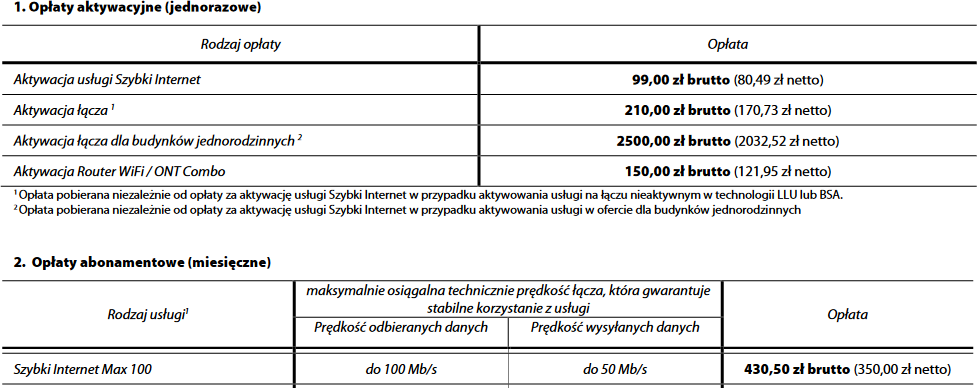
\includegraphics{../pictures/Internet/Netia.png}
	}
\end{figure}
\subsubsection{UPC}
\begin{figure}[H]
	\centering
	\resizebox*{\textwidth}{!}{
		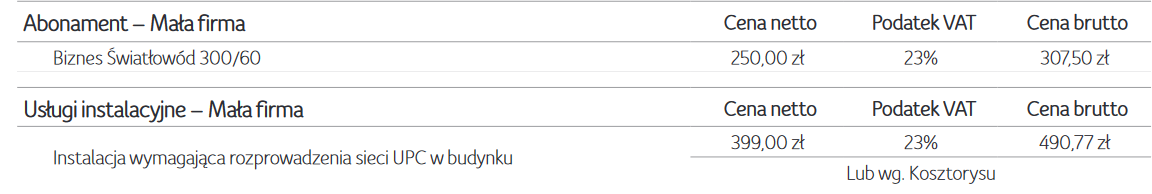
\includegraphics{../pictures/Internet/UPC.png}
	}
\end{figure}
\subsection{Analiza bezpieczeństwa i niezawodności sieci}
\begin{itemize}
	\item Sieć WiFi jest jednym z najbardziej narażonych na atak elementów sieci, dlatego będzie ona szyfrowana za pomocą WPA2.
	\item W sieci zastosowaliśmy VLANy, aby umożliwić logiczne pogrupowanie stacji roboczych.
	\item Każda stacja robocza będzie zabezpieczona firewallem oraz antywirusem.
	\item W przypadku awarii jednego z dostawców Internetu, możemy przekierować ruch na dwóch pozostałych dostawców, co pozwala na stały i bezawaryjny dostęp do Internetu.
	\item Redundancja łącza internetowego oraz zastosowanie niezawodnego sprzętu sieciowego wysokiej jakości pozwala uzyskać niezawodność sieci.
	\item W budynkach zostaną zamontowane zasilacze awaryjne (UPS - uninterruptible power supply), aby pracownicy zdążyli zapisać pracę oraz bezpiecznie wyłączyć
	      urządzenia bądź kontynuować pracę jeżeli zaniki zasilania są chwilowe.
\end{itemize}
\subsection{Kosztorys}
% TODO kosztorys
\begin{table}[H]
	\centering
	\caption{Kosztorys pierwszego roku}
	\begin{tabular}{|llc|c|}
		\hline
		\multicolumn{1}{|c|}{\textbf{Nazwa}}               & \multicolumn{1}{c|}{\textbf{L. sztuk}} & \textbf{Cena [zł]}    & \textbf{Łącznie [zł]}                        \\ \hline
		\multicolumn{1}{|l|}{Cisco 2911/K9}                & \multicolumn{1}{c|}{1}                 & $5,991.81$            & $5,991.81$                                   \\ \hline
		\multicolumn{1}{|l|}{Cisco Catalyst 2960X-24TS-LL} & \multicolumn{1}{c|}{1}                 & $4,220.36$            & $4,220.36$                                   \\ \hline
		\multicolumn{1}{|l|}{Cisco SF350-48}               & \multicolumn{1}{c|}{2}                 & $1,714.06$            & $3,428.12$                                   \\ \hline
		\multicolumn{1}{|l|}{Cisco SF220-48}               & \multicolumn{1}{c|}{20}                & $970.02$              & $19,400.4$                                   \\ \hline
		\multicolumn{1}{|l|}{TP-LINK EAP265 HD}            & \multicolumn{1}{c|}{6}                 & $475.50$              & $2,853$                                      \\ \hline
		\multicolumn{1}{|l|}{Internet Netia}               & \multicolumn{1}{l|}{-}                 & $350.50$ [msc]        & $4,206,00$ [rok]                             \\ \hline
		\multicolumn{1}{|l|}{Instalacja Netia}             & \multicolumn{1}{l|}{1}                 & $170.73$              & $170.73$                                     \\ \hline
		\multicolumn{1}{|l|}{Internet UPC}                 & \multicolumn{1}{l|}{-}                 & $250$ [msc]           & $3,000$ [rok]                                \\ \hline
		\multicolumn{1}{|l|}{Instalacja UPC}               & \multicolumn{1}{l|}{1}                 & $399$                 & $399$                                        \\ \hline
		\textbf{Suma}                                      &                                        & \multicolumn{1}{l|}{} & \multicolumn{1}{r|}{\textbf{$43,699.42$ zł}} \\ \hline
	\end{tabular}
\end{table}

\begin{table}[H]
	\centering
	\caption{Kosztorys lat przyszłych (koszt jednego roku)}
	\begin{tabular}{|lc|c|}
		\hline
		\multicolumn{1}{|c|}{\textbf{Nazwa}} & \textbf{Cena [zł/msc]} & \textbf{Łącznie [zł/rok]} \\ \hline
		\multicolumn{1}{|l|}{Internet Netia} & $350.50$               & $4,206,00$                \\ \hline
		\multicolumn{1}{|l|}{Internet UPC}   & $250$                  & $3,000$                   \\ \hline
		\textbf{Suma}                        & \multicolumn{1}{l|}{}  & \textbf{$7,206$ zł}       \\ \hline
	\end{tabular}
\end{table}

\section{Karty katalogowe proponowanych urządzeń}
\subsection{Router Cisco 2911/K9}
\begin{figure}[H]
	\centering
	\resizebox*{\textwidth}{!}{
		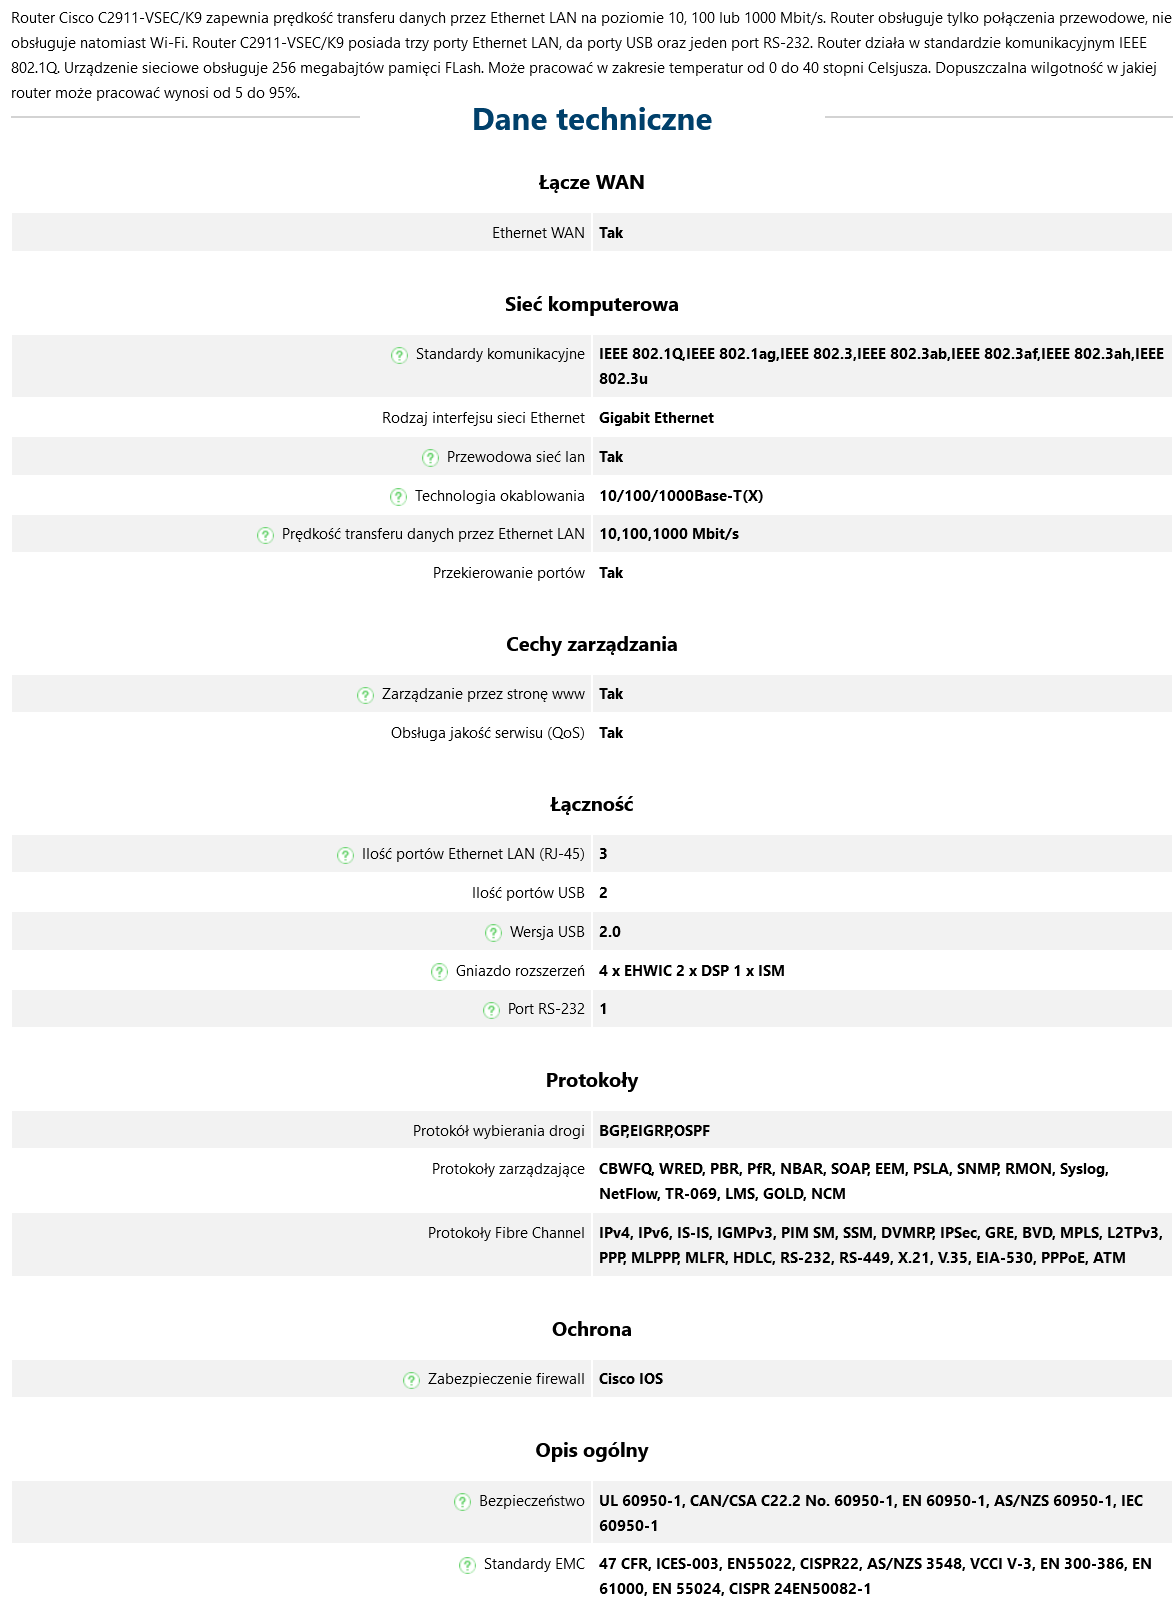
\includegraphics{../pictures/spec-cards/router-Cisco-2911-K9.png}
	}
\end{figure}
\subsection{Switch warstwy 3 Cisco Catalyst 2960X-24TS-LL}
\begin{figure}[H]
	\centering
	\resizebox*{\textwidth}{!}{
		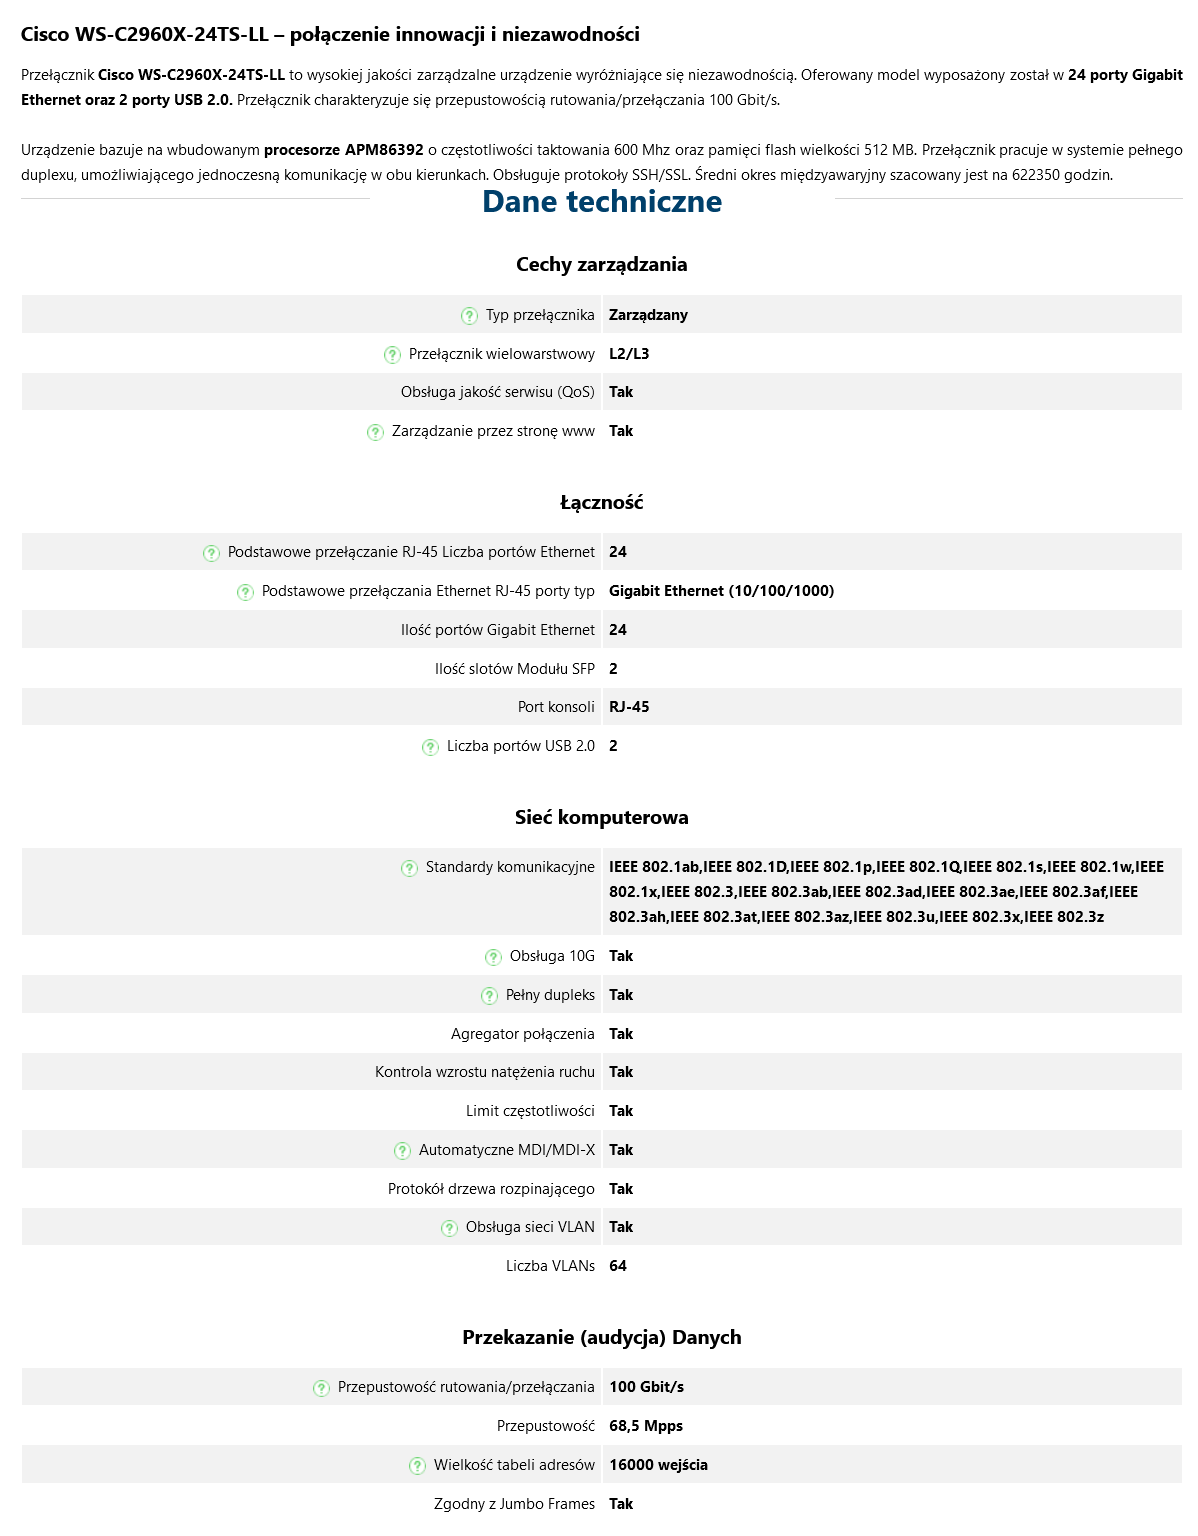
\includegraphics{../pictures/spec-cards/ws-cs2960.png}
	}
\end{figure}
\subsection{Switch warstwy 3 Cisco SF350-48}
\begin{figure}[H]
	\centering
	\resizebox*{\textwidth}{!}{
		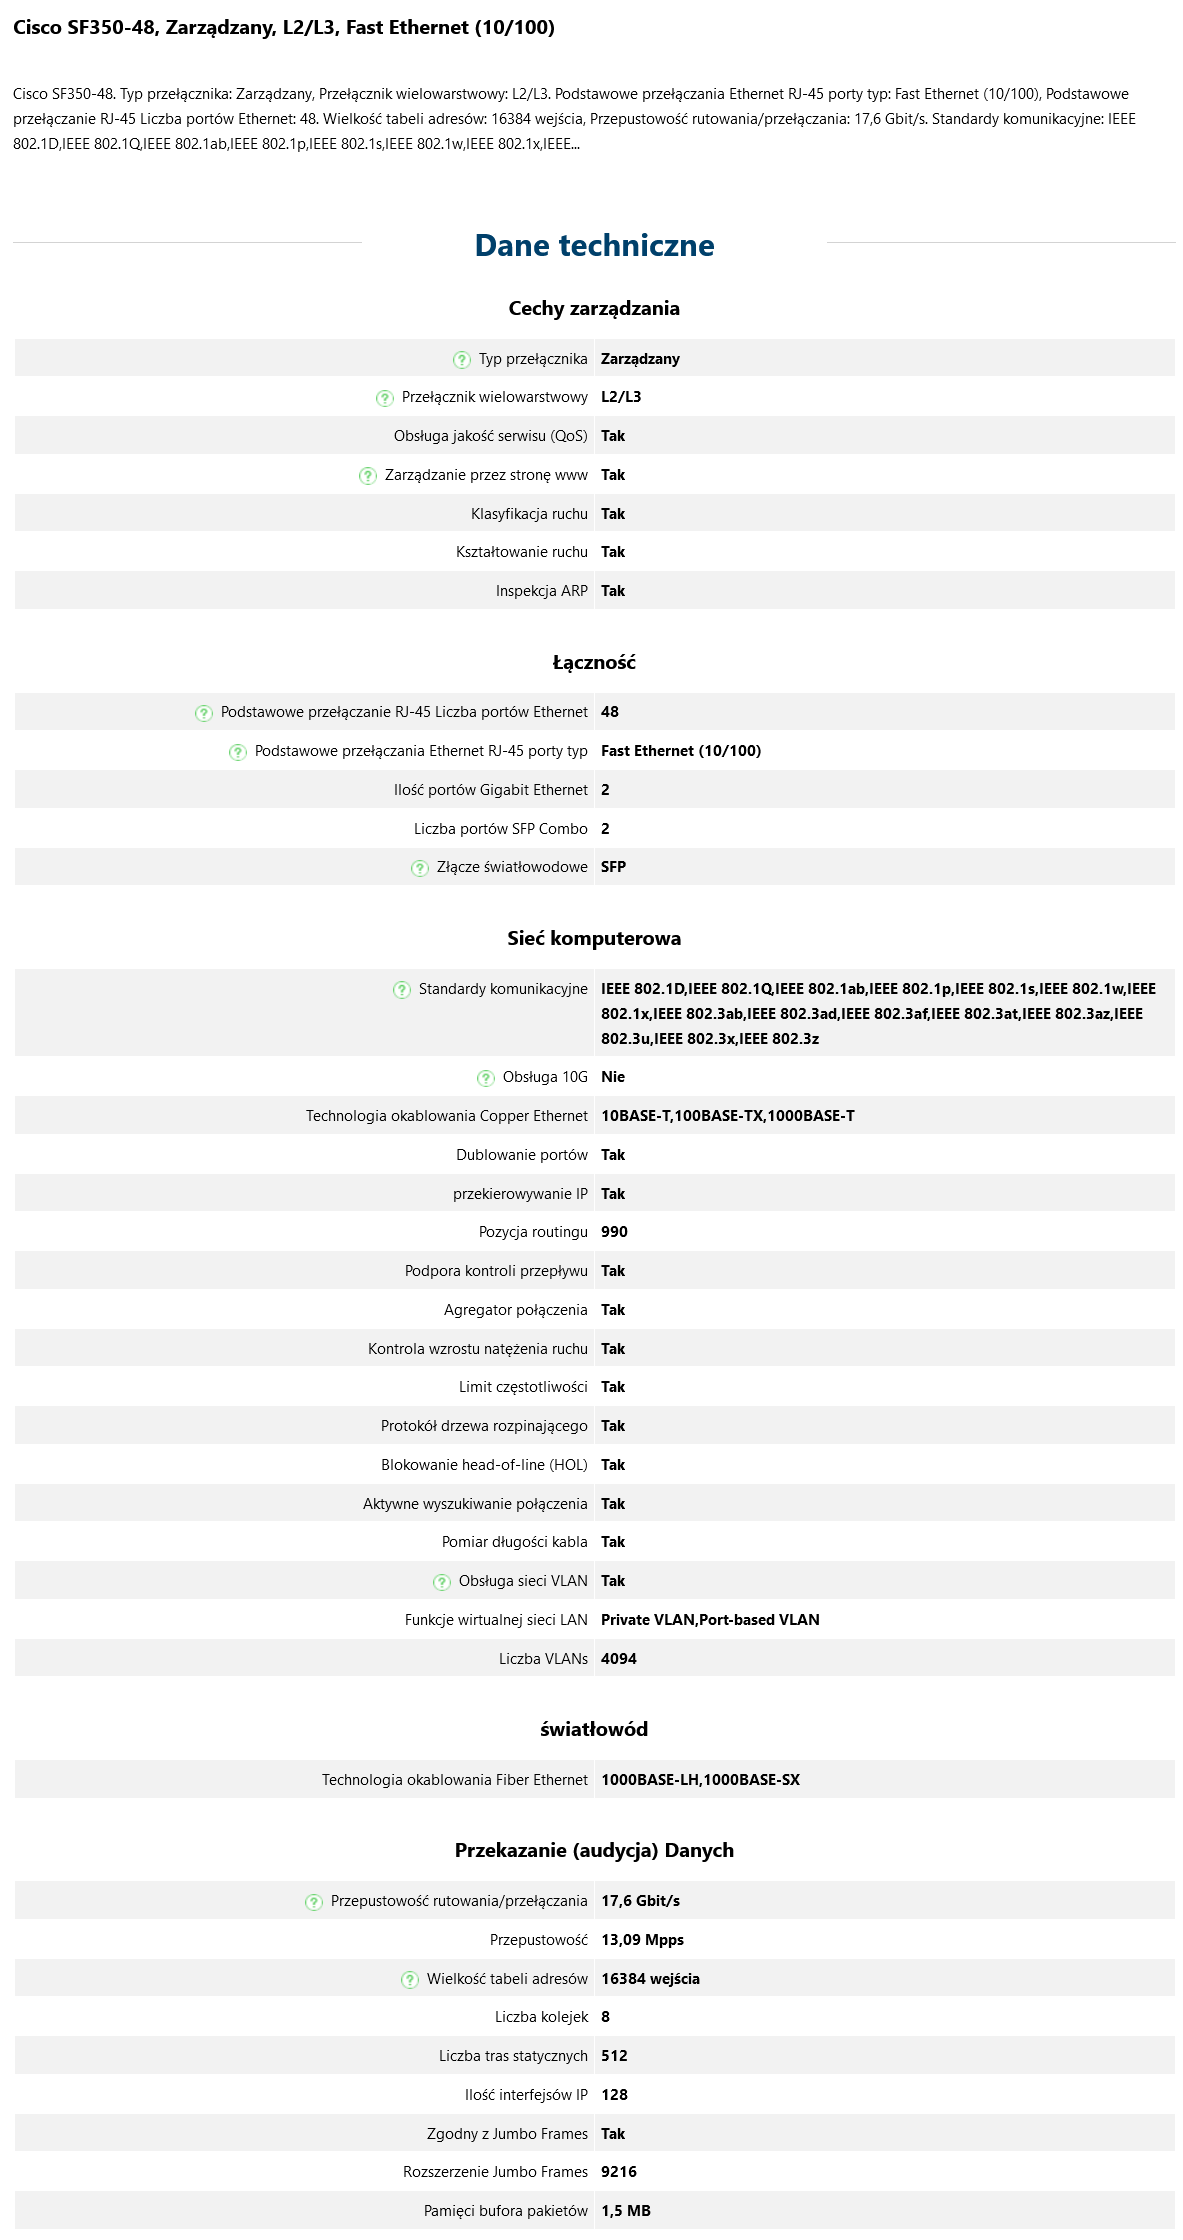
\includegraphics{../pictures/spec-cards/sf350.png}
	}
\end{figure}
\subsection{Switch warstwy 2 Cisco SF220-48}
\begin{figure}[H]
	\centering
	\resizebox*{\textwidth}{!}{
		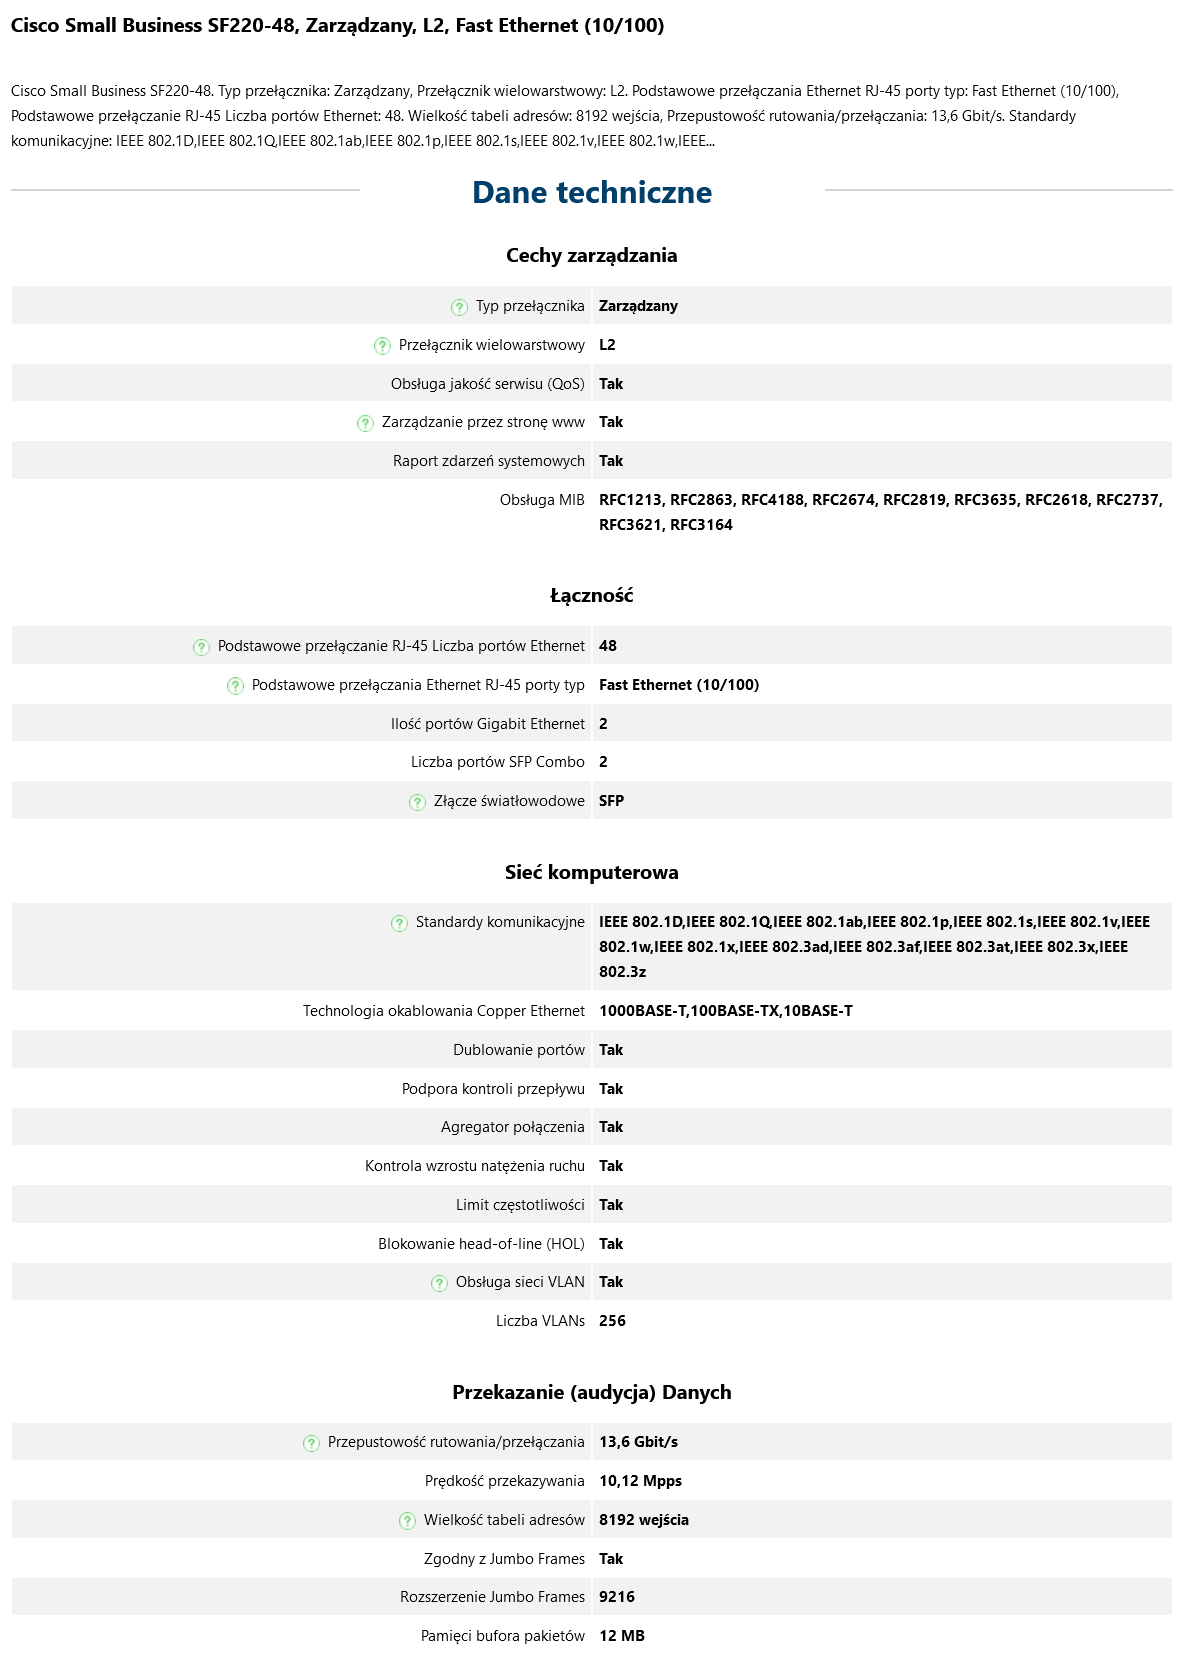
\includegraphics{../pictures/spec-cards/sf220.png}
	}
\end{figure}
\subsection{TP-LINK EAP265 HD}
\begin{figure}[H]
	\centering
	\resizebox*{\textwidth}{!}{
		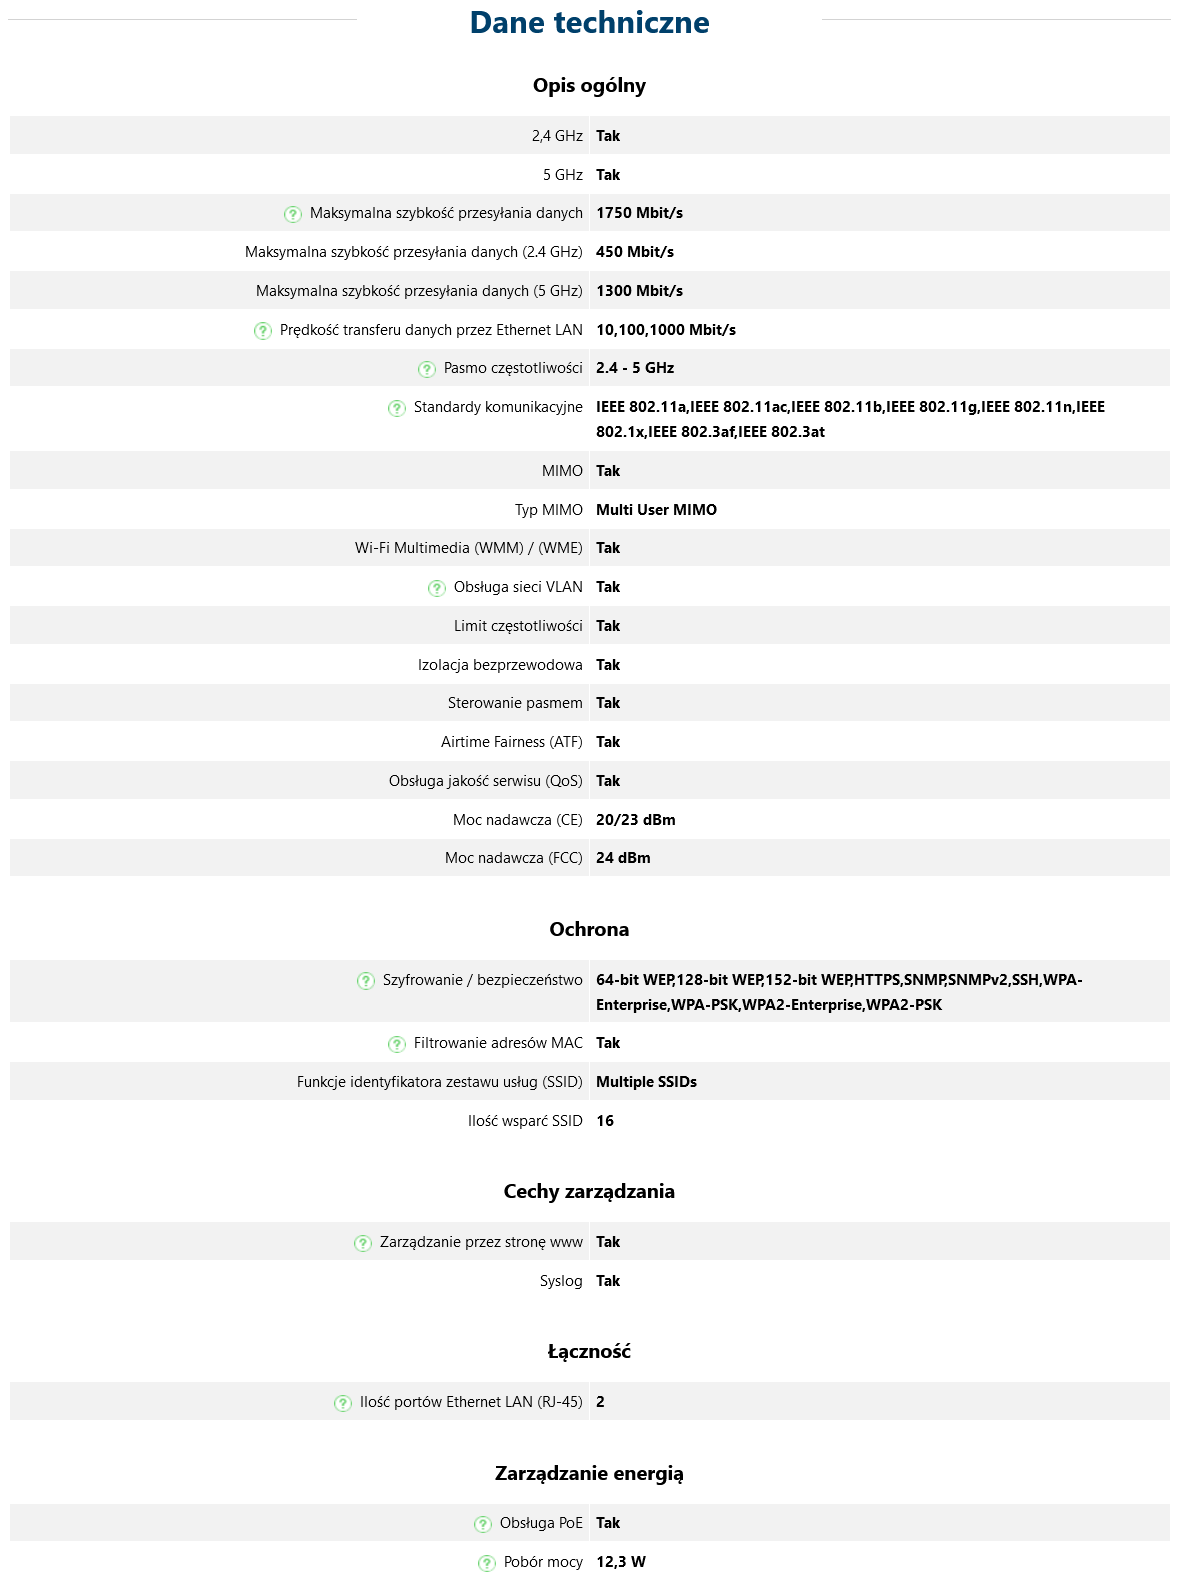
\includegraphics{../pictures/spec-cards/tp-link-eap265hd.png}
	}
\end{figure}
% Router - https://www.cisco.com/c/en/us/support/routers/4221-integrated-services-router-isr/model.html
% Price - 2 765,51 zł netto  3 401,58 zł brutto

% layer 3 - https://www.cisco.com/c/en/us/support/switches/catalyst-2960x-24ts-ll-switch/model.html
% Price -  4 220,36 zł netto  5 191,04 zł brutto 

% layer 3 weaker - https://www.cisco.com/c/en/us/support/switches/sf350-48-48-port-10-100-managed-switch/model.html
% Price -  1 714,06 zł netto 2 108,29 zł brutto 

% layer 2 - https://www.cisco.com/c/en/us/support/switches/sf220-48-48-port-10-100-smart-plus-switch/model.html
% Price -  970,02 zł netto 1 193,12 zł brutto 

% Access point - https://www.senetic.pl/product/EAP265_HD
% Price - 475,50 zł netto 584,87 zł brutto

% Even cheaper alternatives: https://mikrotik.com/
\end{document}
